\documentclass[12pt]{jarticle}
% \documentclass[10.5pt]{jarticle}

% Language setting
% Replace `english' with e.g. `spanish' to change the document language
% \usepackage[english]{babel}
\usepackage[dvipdfmx]{graphicx}
\usepackage[dvipdfmx]{color}

% Set page size and margins
% Replace `letterpaper' with `a4paper' for UK/EU standard size
% \usepackage[letterpaper,top=2cm,bottom=2cm,left=2cm,right=2cm,marginparwidth=1.75cm]{geometry}
\usepackage[letterpaper,top=2cm,bottom=3cm,left=1cm,right=1cm,marginparwidth=1cm]{geometry}

% Useful packages
\usepackage{amsmath}
\usepackage{graphicx}
\usepackage[colorlinks=true, allcolors=blue]{hyperref}
\usepackage{longtable}
\usepackage{amsmath}
\usepackage{booktabs}
\usepackage{breqn}
\usepackage{lscape}
\usepackage{amsmath,amsthm,amssymb,multirow} %カンマで区切ることで一度にusepackageできる
%\usepackage{natbib}
\usepackage{here}
\usepackage{color}
\usepackage{bm}
%\usepackage{subfig}
\usepackage{subcaption}
\usepackage{listings, jlisting}
\usepackage{txfonts}
\usepackage{comment}
\usepackage{ascmac}
\usepackage{algorithm}
\usepackage{algorithmic}
\usepackage{tabularx}

% 数式サイズを大きくする設定
\newcommand{\mathbm}[1]{{\mbox{\boldmath $#1$}}}
\newcommand{\rd}{\partial}
\newcommand{\dd}[2]{\dfrac{\partial #1}{\partial #2}}
\newcommand{\ddd}[2]{\dfrac{\partial^2 #1}{\partial #2^2}}
\newcommand{\dddd}[3]{\dfrac{\partial^2 #1}{\partial #2 \partial #3}}
\newcommand{\ol}{\overline}
\newcommand{\bibname}{参考文献}
\renewcommand{\figurename}{図}
\renewcommand{\tablename}{表}
\renewcommand{\lstlistingname}{ソースコード}
\newcommand{\keywords}[1]{\par\noindent{\small\textbf{キーワード:} #1}\par\vspace{1em}}
\newcommand{\Eqref}[1]{式~(\ref{#1})}
\newcommand{\Figref}[1]{図~\ref{#1}}
\newcommand{\Tblref}[1]{表~\ref{#1}}
\newcommand{\Coderef}[1]{ソースコード~\ref{#1}}
\newcommand{\Algref}[1]{Algorithm~\ref{#1}}
\newcommand{\red}[1]{\textcolor{red}{#1}}
\newcommand{\blue}[1]{\textcolor{blue}{#1}}
% \newcommand{\yellow}[1]{\textcolor{yellow}{#1}}
% \newcommand{\violet}[1]{\textcolor{violet}{#1}}

\theoremstyle{plain}
\newtheorem{thm}{Theorem}
\newtheorem*{thm*}{Theorem}
\theoremstyle{definition}
\newtheorem{dfn}{Definition}

\title{SE(3)上における協調自己位置推定のための\\視野共有を保証する分散型CBF}
\author{滑川研究室\ \ \ M2 有田 朋樹}
\date{\today}

\begin{document}
\maketitle

\begin{abstract}
    This paper proposes a novel distributed probabilistic pose graph filtering framework on SE(3). It integrates ADMM with Stein Variational Gradient Descent (SVGD) to address multi-modal, non-Gaussian posteriors in multi-robot SLAM.
    We reformulate pose graph filtering as Bayesian posterior estimation on SE(3) using particles. The consistency requirement, minimizing KL divergence, is cast into an augmented Lagrangian and decomposed via ADMM. Agents perform local SVGD updates and consensus steps, communicating only summary statistics.
    The proposed method (i) maintains multiple hypotheses for ambiguous loop closures, (ii) reduces communication by exchanging only Lagrange multipliers and particle summaries, and (iii) handles SE(3) nonlinearity. Convergence is proven under standard ADMM conditions, and KL minimization is validated.
    Simulations demonstrate real-time convergence, outlier robustness, and accurate posterior approximation.
\end{abstract}

\begin{keywords}
Probabilistic pose graph filtering; SE(3); ADMM; Stein Variational Gradient Descent; Multi-robot SLAM
\end{keywords}

\section{序論}

\subsection{共有視野保証の重要性と背景}

マルチロボットシステムでは,各ロボットがセンサ情報や視界を共有することにより,監視・捜索・協調輸送などのタスクを効率的に遂行できることが知られている.
特にカメラを用いた視覚協調の場合,各ロボットの共有視野(Common Field-of-View, CoFoV)が不可欠である.例えば,複数ドローンが異なる角度から同一対象を観測できることや,通信の見通し線(LOS)維持が求められる\cite{Panagou2017}.

マルチエージェントVSLAM(Visual Simultaneous Localization and Mapping)においては,各エージェントが撮影した画像から抽出される局所特徴に基づき自己局在を行い,エージェント間で特徴マッチングにより相対位置を推定する.従来のORBやSIFTに代わり,SuperPointのような学習型局所特徴検出・記述器\cite{DeTone2018}や,NetVLADによるグローバル記述子\cite{Arandjelovic2016}が高いロバスト性を示し,ループ検出やキーフレームマッチングに貢献している.

画像特徴量のマッチングを成功させるためには,各エージェントが共通のランドマークを観測できるよう,カメラの視野錐台の幾何学的重複が必要である.視野重複が存在すれば,エージェント間でのループ検出が可能となり,その結果として各ロボットの地図統合が実現される\cite{Zhang2022}.しかし,ロボットは視野角が限られているため,視界共有を保証するための制御技術の開発が急務である.

\red{モチベーション:CoVINSではsuperpoint特徴量などの画像特徴量のマッチングにより、自己位置推定に関する最適化問題のfactorを得ている。特徴量をマッチングするにはエージェントの視野錐台が重なっている必要がある。single agent問題に関してはstereo cameraの相対位置をconstかつgivenとして最適化問題に組み込み、multi agent問題に関しては視野錐台のoverrideは不可知であるために画像全体特徴量の類似度の一致などによってpassiveなevent trigger型としてアルゴリズムが構築されている。しかし、agent1とagent2が視野錐台を交差させ続けるための制御則(CBF等)に基づいてactive perceptionを行う場合、multi agentの自己位置推定においてinter-agentな特徴量のマッチング及び推定問題はエージェントをまたいだカメラ間の相対位置をgiven, もしくは最適化すべき双対変数として複数のエージェント位置を同時最適化できるはずである。さらに、active perceptionの枠組みで考えれば、CBFを用いた最適制御問題と自己位置推定問題も同一の目的関数の最小化問題として扱うことができるはずである。  
上記の仮定から、本セミナーではその手始めとして,代表的なCoVINSであるUAVを対象として、視野錐台を交差させ続けるための分散型CBF手法を提案する。}

\begin{figure}[htbp]
\centering
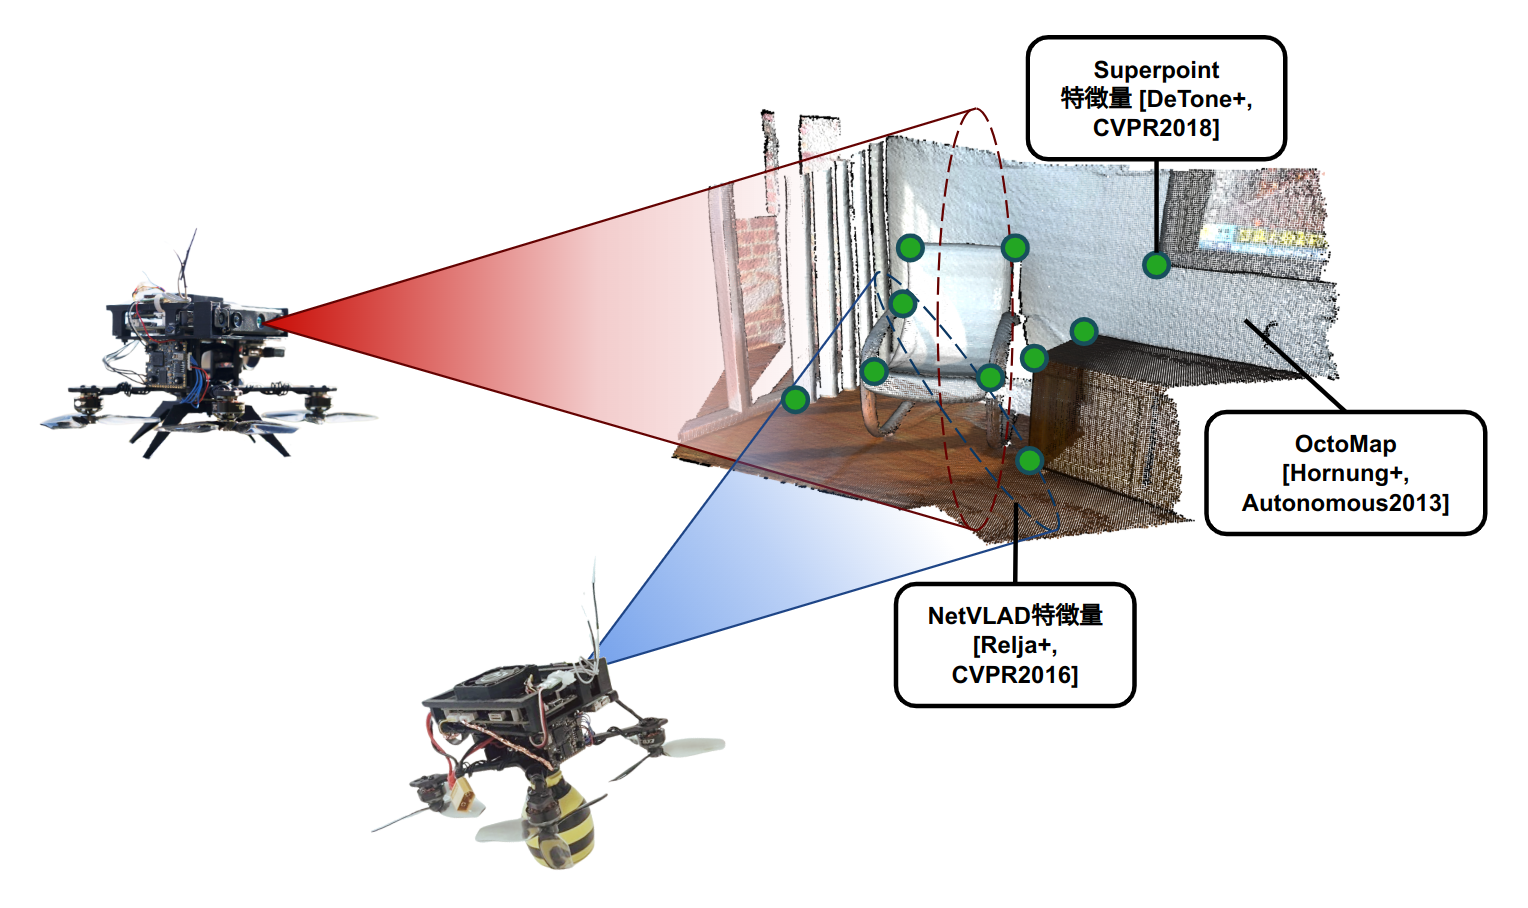
\includegraphics[width=0.8\linewidth]{fig/covins.png}
\caption{COVINSの構成}
\label{fig:covins}
\end{figure}
\subsection{既存研究の課題}

従来はポテンシャル場やMPC(Model Predictive Control)を用いた手法が提案され,局所的な視界制約下での隊列制御やセンサグラフの連結性維持に取り組まれてきた\cite{Sabattini2013}.一方で,制御バリア関数(Control Barrier Function, CBF)を用いた手法は,制約違反を防ぎながらリアルタイムに最適な制御入力を計算できるため,有力な候補となる\cite{Capelli2020}.

しかし,現状の協調SLAMは,キーフレームの受動的な共有と画像類似度評価に依存しており,視野重複が偶発的に発生しなければマップ統合が成立しないリスクがある.また,多数のロボットを対象とする場合,中央集権的な制御は通信負荷や計算量の面で現実的ではなく,各エージェントが局所的に計算し,限定的な通信で連携する分散アルゴリズムの設計が必要である.

従来の視野維持手法は,対象が視野内にあるか否かを決定論的に評価するに留まっていたが,センサの観測不確実性を十分に取り入れていなかった\cite{Panagou2012}.また,従来の多くの視野制約付き制御手法は,単純な動力学モデル(例:Dubins車両やクアッドロータの水平姿勢維持)に基づいており,非ホロノミックなダイナミクスを明示的に考慮していなかった\cite{Dias2016}.

\subsection{本研究の貢献}

本研究では,SE(3)上における協調自己位置推定のための視野共有を保証する分散型CBF手法を提案する.本研究の主な貢献は以下の通りである.

\begin{itemize}
\item SE(3)における共有視野保証を実現する.従来のステレオ視やリーダーフォロワ形式による視野制御は,ロボット間の相対配置を幾何学的に制約するに留まっていたが,本手法は3次元空間におけるエージェント全体の姿勢・位置を統合的に制御する枠組みを提供する.

\item 特徴点に基づく確率的可視性制約とCBFの適用を行う.本研究では,各エージェントが観測する特徴点に基づき,その可視性を確率的に評価した上で,CBFに組み込み,常時高い確率で共有視野が確保されるよう制御入力を設計する.これにより,センサノイズ等による不確実性下でも安全な視野維持が可能となる.

\item 非ホロノミックなドローンダイナミクスへの対応と分散最適化を実現する.本研究では,機体の並進および回転運動を同時に考慮するSE(3)上の非ホロノミックドローンモデルに対して,高次制約も扱える高次制御バリア関数(HOCBF)を導入し,各エージェントが局所的な情報交換を通じて分散最適化アルゴリズム(PDMM等)により制御解を求める枠組みを提案する\cite{Lv2024}.これにより,リアルタイム性とスケーラビリティの両立を実現する.
\end{itemize}

\subsection{論文構成}

本論文の構成は以下の通りである.第2章ではCBFの基本概念と高次CBFについて説明する.第3章では問題設定とシステムモデルについて述べる.第4章では共有視野のためのCBFを提案し,第5章では二次系システムのための高次CBFを導入する.第6章ではシミュレーション結果を示し,第7章で結論と今後の課題について述べる.

\begin{figure}[htbp]
\centering
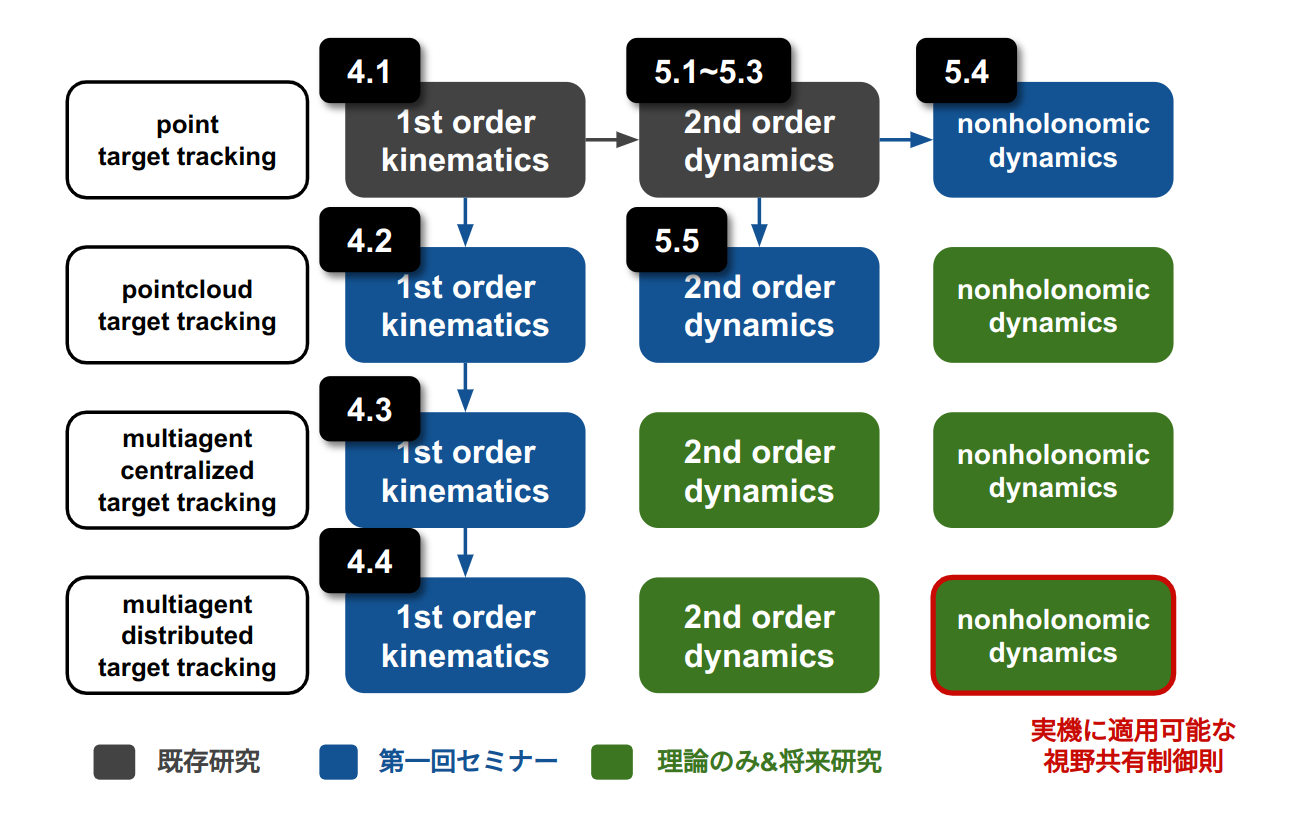
\includegraphics[width=0.8\linewidth]{fig/progress.png}
\caption{第一回セミナーの内容と本研究の貢献点}
\label{fig:progress}
\end{figure}
% \section{\textbf{準備:制御バリア関数}}
\section{準備:制御バリア関数}

本章では,本研究の基礎となる制御バリア関数(Control Barrier Function, CBF)の基本概念と高次制御バリア関数(High Order Control Barrier Function, HOCBF)について説明する.

\subsection{CBFの基本概念}

CBFは,システム状態がある安全集合内に留まることを保証するためのLyapunov関数に類似した概念である.以下では,CBFの基本的な定義と性質について述べる.

連続時間の制御アフィンシステムを考える:
\begin{equation}
\begin{aligned}
\dot{\mathbf{x}} = f(\mathbf{x}) + g(\mathbf{x})\mathbf{u}
\label{eq:control_affine}
\end{aligned}
\end{equation}
ここで,$\mathbf{x} \in \mathbb{R}^n$は状態,$\mathbf{u} \in \mathbb{R}^m$は制御入力,$f: \mathbb{R}^n \rightarrow \mathbb{R}^n$と$g: \mathbb{R}^n \rightarrow \mathbb{R}^{n \times m}$は局所Lipschitz連続な関数である.

安全集合$\mathcal{C}$を以下のように定義する:
\begin{equation}
\begin{aligned}
\mathcal{C} = \{\mathbf{x} \in \mathbb{R}^n : h(\mathbf{x}) \geq 0\}
\label{eq:safe_set}
\end{aligned}
\end{equation}
ここで,$h: \mathbb{R}^n \rightarrow \mathbb{R}$は連続微分可能な関数である.

\begin{dfn}[制御バリア関数]
関数$h: \mathbb{R}^n \rightarrow \mathbb{R}$が連続微分可能であり,その勾配$\nabla h(\mathbf{x})$が$\mathcal{C}$上でゼロにならないとする.このとき,$h$が制御バリア関数であるとは,ある拡張クラス$\mathcal{K}_{\infty}$関数$\alpha$が存在して,任意の$\mathbf{x} \in \mathcal{C}$に対して以下の条件を満たす制御入力$\mathbf{u} \in \mathbb{R}^m$が存在することである:
\begin{equation}
\begin{aligned}
L_f h(\mathbf{x}) + L_g h(\mathbf{x})\mathbf{u} + \alpha(h(\mathbf{x})) \geq 0
\label{eq:cbf_condition}
\end{aligned}
\end{equation}
ここで,$L_f h(\mathbf{x}) = \nabla h(\mathbf{x})^T f(\mathbf{x})$と$L_g h(\mathbf{x}) = \nabla h(\mathbf{x})^T g(\mathbf{x})$はそれぞれ$h$の$f$と$g$に関するLie微分である.
\end{dfn}

CBFの重要な性質は,\Eqref{eq:cbf_condition}を満たす任意の制御入力$\mathbf{u}$を用いると,安全集合$\mathcal{C}$が前方不変となることである.つまり,初期状態$\mathbf{x}(0) \in \mathcal{C}$に対して,任意の時刻$t \geq 0$において$\mathbf{x}(t) \in \mathcal{C}$が保証される.

実際の制御設計では,CBF制約を満たしつつ,制御目標を達成するための最適制御入力を求めることが多い.これは以下のような二次計画問題(Quadratic Programming, QP)として定式化できる:
\begin{equation}
\begin{aligned}
\mathbf{u}^* &= \underset{\mathbf{u} \in \mathbb{R}^m}{\text{argmin}} \:\: \|\mathbf{u} - \mathbf{u}_{\text{nom}}\|^2 \\
\text{s.t.} & \:\: L_f h(\mathbf{x}) + L_g h(\mathbf{x})\mathbf{u} + \alpha(h(\mathbf{x})) \geq 0
\label{eq:cbf_qp}
\end{aligned}
\end{equation}
ここで,$\mathbf{u}_{\text{nom}}$は安全制約を考慮しない場合の公称制御入力である.

\subsection{高次制御バリア関数}

従来のCBFは制約関数の相対次数が1であることを仮定していたが,多くの実システムでは安全制約が高次微分に依存するため,高次制御バリア関数(HOCBF)が必要となる.

関数$h(\mathbf{x})$の相対次数が$r > 1$の場合,以下のように補助関数の連鎖を定義する:
\begin{equation}
\begin{aligned}
\psi_0(\mathbf{x}) &= h(\mathbf{x}) \\
\psi_1(\mathbf{x}) &= \dot{\psi}_0(\mathbf{x}) + \alpha_1(\psi_0(\mathbf{x})) \\
\psi_2(\mathbf{x}) &= \dot{\psi}_1(\mathbf{x}) + \alpha_2(\psi_1(\mathbf{x})) \\
&\vdots \\
\psi_{r-1}(\mathbf{x}) &= \dot{\psi}_{r-2}(\mathbf{x}) + \alpha_{r-1}(\psi_{r-2}(\mathbf{x}))
\label{eq:hocbf_psi}
\end{aligned}
\end{equation}
ここで,$\alpha_i$($i = 1, 2, \ldots, r-1$)は拡張クラス$\mathcal{K}$関数である.

\begin{dfn}[高次制御バリア関数]
関数$h: \mathbb{R}^n \rightarrow \mathbb{R}$が$r$回連続微分可能であり,その相対次数が$r$であるとする.このとき,$h$が高次制御バリア関数であるとは,拡張クラス$\mathcal{K}$関数$\alpha_1, \alpha_2, \ldots, \alpha_r$が存在して,以下の条件を満たすことである:
\begin{equation}
\begin{aligned}
L_f^r h(\mathbf{x}) + L_g L_f^{r-1} h(\mathbf{x})\mathbf{u} + \alpha_r(\psi_{r-1}(\mathbf{x})) \geq 0
\label{eq:hocbf_condition}
\end{aligned}
\end{equation}
ここで,$L_f^r h(\mathbf{x})$は$h$の$f$に関する$r$次のLie微分,$L_g L_f^{r-1} h(\mathbf{x})$は$L_f^{r-1} h(\mathbf{x})$の$g$に関するLie微分である.
\end{dfn}

HOCBFを用いた制御設計では,\Eqref{eq:hocbf_condition}の制約を満たす制御入力を求めることで,安全集合$\mathcal{C}$の前方不変性を保証できる.これは以下のようなQP問題として定式化できる:
\begin{equation}
\begin{aligned}
    \mathbf{u}^* &= \underset{\mathbf{u} \in \mathbb{R}^m}{\text{argmin}} \:\: \|\mathbf{u} - \mathbf{u}_{\text{nom}}\|^2 \\
\text{s.t.} & \:\:  L_f^r h(\mathbf{x}) + L_g L_f^{r-1} h(\mathbf{x})\mathbf{u} + \alpha_r(\psi_{r-1}(\mathbf{x})) \geq 0
\label{eq:hocbf_qp}
\end{aligned}
\end{equation}

HOCBFは,非ホロノミック制約を持つシステムや,高次の安全制約を持つシステムに対して有効である.特に,本研究で扱うSE(3)上の剛体運動制御では,視野制約が状態の高次微分に依存するため,HOCBFが重要な役割を果たす.

\section{Problem Formulation}
\label{sec:problem_formulation}

This section formally defines the multi-agent pose graph filtering problem addressed in this paper. We begin by establishing the notation used for representing poses and transformations on the Special Euclidean group SE(3), followed by the deterministic and probabilistic formulations of the pose graph filtering problem.

\subsection{Notation on SE(3)}
\label{subsec:notation_se3}

We represent the state (pose) of an agent $i$ at time $t$ as an element of the Special Euclidean group SE(3), denoted by $X_i^t \in \text{SE}(3)$. SE(3) is the group of rigid body transformations in three-dimensional space, combining rotation and translation. An element $X \in \text{SE}(3)$ can be represented by a $4 \times 4$ homogeneous transformation matrix:
\begin{equation}
\begin{aligned}
X =
\begin{pmatrix}
{\mathbf{R}} & {\mathbf{t}} \\
{\mathbf{0}}^{\top} & 1
\end{pmatrix} \in {\mathbb{R}}^{4\times4},
\label{eq:se3_matrix_form}
\end{aligned}
\end{equation}
where ${\mathbf{R}} \in \text{SO}(3)$ is a $3 \times 3$ rotation matrix representing the orientation, and ${\mathbf{t}} \in {\mathbb{R}}^3$ is the translation vector representing the position. SO(3) is the Special Orthogonal group, the space of $3 \times 3$ orthogonal matrices with determinant +1.

The Lie algebra associated with SE(3) is denoted by ${\mathfrak{se}}(3)$. It is the tangent space to the identity element of SE(3) and represents infinitesimal transformations (velocities). An element $\boldsymbol{\xi} \in {\mathfrak{se}}(3)$ is a 6-dimensional vector, often called a twist, composed of translational and rotational velocity components: $\boldsymbol{\xi} = (\boldsymbol{\nu}^{\top}, \boldsymbol{\omega}^{\top})^{\top}$, where $\boldsymbol{\nu} \in {\mathbb{R}}^3$ is the translational velocity and $\boldsymbol{\omega} \in {\mathbb{R}}^3$ is the rotational velocity.

We use the hat operator $(\cdot)^{\wedge}$ to map elements from the vector space ${\mathbb{R}}^6$ to the Lie algebra ${\mathfrak{se}}(3)$ represented as $4 \times 4$ matrices:
\begin{equation}
\begin{aligned}
\boldsymbol{\xi}^{\wedge} =
\begin{pmatrix}
\boldsymbol{\omega}^{\wedge} & \boldsymbol{\nu} \\
{\mathbf{0}}^{\top} & 0
\end{pmatrix} \in {\mathbb{R}}^{4\times4},
\label{eq:se3_hat_operator}
\end{aligned}
\end{equation}
where $\boldsymbol{\omega}^{\wedge}$ is the skew-symmetric matrix corresponding to the rotational velocity vector $\boldsymbol{\omega} \in {\mathbb{R}}^3$:
\begin{equation}
\begin{aligned}
\boldsymbol{\omega}^{\wedge} =
\begin{pmatrix}
0 & -\omega_z & \omega_y \\
\omega_z & 0 & -\omega_x \\
-\omega_y & \omega_x & 0
\end{pmatrix} \in {\mathfrak{so}}(3).
\label{eq:so3_hat_operator}
\end{aligned}
\end{equation}
Here, ${\mathfrak{so}}(3)$ is the Lie algebra of SO(3).

The exponential map $\exp: {\mathfrak{se}}(3) \to \text{SE}(3)$ maps an element from the Lie algebra to the Lie group. For $\boldsymbol{\xi} = (\boldsymbol{\nu}^{\top}, \boldsymbol{\omega}^{\top})^{\top} \in {\mathfrak{se}}(3)$, the exponential map is given by:
\begin{equation}
\begin{aligned}
\exp(\boldsymbol{\xi}^{\wedge}) =
\begin{pmatrix}
\exp(\boldsymbol{\omega}^{\wedge}) & {\mathbf{V}}(\boldsymbol{\omega}) \boldsymbol{\nu} \\
{\mathbf{0}}^{\top} & 1
\end{pmatrix} \in \text{SE}(3),
\label{eq:se3_exp_map}
\end{aligned}
\end{equation}
where $\exp(\boldsymbol{\omega}^{\wedge}) \in \text{SO}(3)$ is the matrix exponential for rotations (Rodrigues' formula), and ${\mathbf{V}}(\boldsymbol{\omega})$ is a $3 \times 3$ matrix:
\begin{equation}
\begin{aligned}
\exp(\boldsymbol{\omega}^{\wedge}) &= {\mathbf{I}}_3 + \frac{\sin \theta}{\theta } \boldsymbol{\omega}^{\wedge} + \frac{1-\cos \theta }{\theta^2}(\boldsymbol{\omega}^{\wedge})^2, \\
{\mathbf{V}}(\boldsymbol{\omega}) &= {\mathbf{I}}_3 + \frac{1-\cos\theta}{\theta^2}\boldsymbol{\omega}^{\wedge} + \frac{\theta-\sin \theta}{\theta^3}(\boldsymbol{\omega}^{\wedge})^2,
\label{eq:so3_exp_and_V}
\end{aligned}
\end{equation}
with $\theta = \|\boldsymbol{\omega}\|$.

The inverse operation, the logarithm map $\log: \text{SE}(3) \to {\mathfrak{se}}(3)$, maps an element from the group back to the algebra. The vee operator $(\cdot)^{\vee}$ maps elements from the matrix representation of the Lie algebra back to the vector space ${\mathbb{R}}^6$. These operations allow us to represent differences between poses in the tangent space. For two poses $X_1, X_2 \in \text{SE}(3)$, their relative transformation is $X_{12} = X_1^{-1} X_2$. The difference in the tangent space at the identity is $\boldsymbol{\xi}_{12} = (\log(X_{12}))^{\vee}$.

\subsection{Probabilistic Problem Formulation for PGF}
\label{subsec:probabilistic_pgo}

The Pose Graph Filtering (PGF) problem aims to estimate the set of poses ${\mathbf{X}} = \{X_i\}_{i \in {\mathcal{V}}}$ for a collection of agents or time steps (nodes ${\mathcal{V}}$ in the graph), given a set of relative pose measurements ${\tilde{Z}}_{ij}$ between pairs of poses $(i, j) \in {\mathcal{E}}$ (edges ${\mathcal{E}}$ in the graph). These measurements typically come from odometry or loop closures. Each measurement ${\tilde{Z}}_{ij} \in \text{SE}(3)$ represents the measured transformation from pose $X_i$ to pose $X_j$. The error $E_{ij}(X_i, X_j) = {\tilde{Z}}_{ij}^{-1} (X_i^{-1} X_j)$ represents the discrepancy.

From a probabilistic perspective, PGF aims to estimate the posterior $P({\mathbf{X}} | {\mathbf{Z}})$ 
of poses${\mathbf{X}}$ given measurements ${\mathbf{Z}} = \{{\tilde{Z}}_{ij}\}$. Assuming independent Gaussian errors $\log(E_{ij}(X_i,X_j))^{\vee} \sim {\mathcal{N}}({\mathbf{0}}, \Sigma_{ij})$, the likelihood $P({\tilde{Z}}_{ij} | X_i, X_j) \propto \exp( -\frac{1}{2} \| \log({\tilde{Z}}_{ij}^{-1} X_i^{-1} X_j)^{\vee} \|^2_{\Omega_{ij}} )$.
The total likelihood is $P({\mathbf{Z}} | {\mathbf{X}}) = \prod P({\tilde{Z}}_{ij} | X_i, X_j)$.
By Bayes' theorem, $P({\mathbf{X}} | {\mathbf{Z}}) \propto P({\mathbf{Z}} | {\mathbf{X}}) P({\mathbf{X}})$.
The Maximum A Posteriori (MAP) estimate ${\mathbf{X}}^*_{MAP}$ maximizes $P({\mathbf{X}} | {\mathbf{Z}})$, or equivalently minimizes:
\begin{equation}
\begin{aligned}
J_{MAP}({\mathbf{X}}) = \frac{1}{2} \sum_{(i,j) \in {\mathcal{E}}} \| \log({\tilde{Z}}_{ij}^{-1} X_i^{-1} X_j)^{\vee} \|^2_{\Omega_{ij}} - \log P({\mathbf{X}}).
\label{eq:map_estimation_min_pgf}
\end{aligned}
\end{equation}
With a uniform prior $P({\mathbf{X}})$, this reduces to a nonlinear least-squares problem.
Standard PGF finds the posterior mode, discarding uncertainty. A more general approach approximates the full posterior $P({\mathbf{X}} | {\mathbf{Z}})$ by finding $q({\mathbf{X}})$ that minimizes the Kullback-Leibler (KL) divergence:
\begin{equation}
\begin{aligned}
q^*({\mathbf{X}}) = \underset{q \in {\mathcal{Q}}}{\arg\min} \, D_{KL}(q({\mathbf{X}}) \| P({\mathbf{X}} | {\mathbf{Z}})).
\label{eq:kl_min_objective}
\end{aligned}
\end{equation}
Minimizing the KL divergence is equivalent to minimizing the variational free energy ${\mathcal{F}}[q]$ (since the evidence $P({\mathbf{Z}})$ is constant w.r.t. $q$):
\begin{equation}
\begin{aligned}
D_{KL}(q \| P) % &= \int q({\mathbf{X}}) \log \frac{q({\mathbf{X}})}{P({\mathbf{X}} | {\mathbf{Z}})} d{\mathbf{X}} \\
% &= -{\mathcal{H}}[q] + \mathbb{E}_q[-\log P({\mathbf{Z}} | {\mathbf{X}}) - \log P({\mathbf{X}})] + \log P({\mathbf{Z}}) \\
&= {\mathcal{F}}[q] + \log P({\mathbf{Z}}), \\
\text{where} \quad {\mathcal{F}}[q] &= \mathbb{E}_q[-\log P({\mathbf{Z}} | {\mathbf{X}}) - \log P({\mathbf{X}})] - {\mathcal{H}}[q].
\label{eq:kl_free_energy}
\end{aligned}
\end{equation}
Here, ${\mathcal{H}}[q] = -\int q({\mathbf{X}}) \log q({\mathbf{X}}) d{\mathbf{X}}$ is the entropy of the distribution $q$. Assuming a uniform prior $P({\mathbf{X}})$ and using the likelihood definition described earlier (leading to the MAP formulation in \Eqref{eq:map_estimation_min_pgf}), the term $-\log P({\mathbf{Z}} | {\mathbf{X}})$ corresponds to the PGF cost function (up to constants):
\begin{equation}
\begin{aligned}
C({\mathbf{X}}) = \frac{1}{2} \sum_{(i,j) \in {\mathcal{E}}} \| \log({\tilde{Z}}_{ij}^{-1} X_i^{-1} X_j)^{\vee} \|^2_{\Omega_{ij}}.
\label{eq:cost_function_C}
\end{aligned}
\end{equation}
Thus, minimizing the KL divergence becomes equivalent to minimizing the free energy, which involves a trade-off between minimizing the expected cost and maximizing the entropy:
\begin{equation}
\begin{aligned}
\min_q {\mathcal{F}}[q] = \min_q \left( \mathbb{E}_q[C({\mathbf{X}})] - {\mathcal{H}}[q] \right).
\label{eq:kl_min_cost_entropy}
\end{aligned}
\end{equation}
This formulation seeks a distribution $q$ that concentrates on low-cost configurations (low $\mathbb{E}_q[C({\mathbf{X}})]$) while maximizing entropy ${\mathcal{H}}[q]$ (representing uncertainty).

% The standard MAP estimation \Eqref{eq:map_estimation_min_pgf} can be recovered as a special case of this KL minimization framework. If we restrict the approximating distribution $q({\mathbf{X}})$ to be a Dirac delta function centered at a single point ${\mathbf{X}}_0$, i.e., $q({\mathbf{X}}) = \delta({\mathbf{X}} - {\mathbf{X}}_0)$, then the entropy term ${\mathcal{H}}[q]$ becomes negative infinity (or is undefined, but its contribution vanishes in the limit). The expectation $\mathbb{E}_q[C({\mathbf{X}})]$ simply evaluates the cost function at ${\mathbf{X}}_0$, i.e., $\mathbb{E}_q[C({\mathbf{X}})] = C({\mathbf{X}}_0)$. In this case, minimizing the free energy (ignoring the problematic entropy term) reduces to minimizing $C({\mathbf{X}}_0)$, which is exactly the deterministic PGF problem \Eqref{eq:deterministic_pgf_final} (equivalent to MAP estimation with a uniform prior). Therefore, the deterministic formulation finds a single point estimate by implicitly using a Dirac delta approximation within the broader probabilistic framework of KL divergence minimization. Our work, detailed in the following sections, focuses on using more expressive non-parametric distributions for $q({\mathbf{X}})$ to capture the full posterior uncertainty.

\section{共有視野のためのCBF}

本章では,共有視野を保証するための制御バリア関数(CBF)を設計する.まず単一の特徴点を追従する場合の安全制約を導出し,次に複数の特徴点を追従する場合,さらに複数のエージェントが共通の特徴点を追従する場合へと拡張する.最後に,分散型実装について述べる.

\subsection{単一特徴点追従の安全制約}

単一の特徴点$q_l \in \mathcal{L}$を追従する安全制約について考える.前章で述べたように,特徴点$q_l$がエージェント$i$の視野内にある条件は以下のように表される:
\begin{equation}
\begin{aligned}
q_l \in \mathcal{C}_i \iff \beta_l^{\top}(p_i)R_ie_c - \cos\Psi_{\mathcal{F}} > 0
\label{eq:single_fov_condition}
\end{aligned}
\end{equation}

この条件に基づいて,安全集合を以下のように定義する:
\begin{equation}
\begin{aligned}
B_i = \beta_l^{\top}(p_i)R_ie_c - \cos\Psi_{\mathcal{F}}
\label{eq:single_safe_set}
\end{aligned}
\end{equation}

CBFの条件を適用するためには,$B_i$の時間微分を計算する必要がある.$B_i$の時間微分は以下のように計算できる:
\begin{equation}
\begin{aligned}
\dot{B}_i &= \langle \mathrm{grad}_R\:B_i, \omega_i \rangle + \langle \mathrm{grad}_p\:B_i, v_i \rangle \\
&= -\beta_l^\top(p_i) R_i [e_c]_\times\omega_i - \frac{e_c^\top R_i^\top P_{\beta_l}}{d_{i,l}}v_i
\label{eq:single_cbf_derivative}
\end{aligned}
\end{equation}
ここで,$d_{i,l} = \|q_l-p_i\|$は特徴点$q_l$とエージェント$i$の距離,$P_{\beta_l} = I - \beta_l\beta_l^\top$は$\beta_l$に直交する平面への投影行列である.

CBFの条件より,安全制約は以下のように表される:
\begin{equation}
\begin{aligned}
-\beta_l^\top(p_i) R_i [e_c]_\times\omega_i - \frac{e_c^\top R_i^\top P_{\beta_l}}{d_{i,l}}v_i \leq \gamma (B_i)
\label{eq:single_cbf_constraint}
\end{aligned}
\end{equation}
ここで,$\gamma$は拡張クラス$\mathcal{K}$関数であり,通常は$\gamma(B_i) = \gamma_0 B_i$($\gamma_0 > 0$は定数)のように線形関数を用いる.

CBF制約を満たしつつ,目標位置$p_i^d$に追従するためのQP問題は以下のように定式化できる:
\begin{equation}
\begin{aligned}
\min_{\xi_i} \quad & (p^d_i - p_i - hv_i)^\top Q_1 (p^d_i - p_i - hv_i) + \xi_i^\top Q_2 \xi_i \\
\mathrm{s.t.} \quad & -\beta_l^\top(p_i) R_i [e_c]_\times\omega_i - \frac{e_c^\top R_i^\top P_{\beta_l}}{d_{i,l}}v_i \leq \gamma_0 (\beta_l^{\top}(p_i)R_ie_c - \cos\Psi_{\mathcal{F}})
\label{eq:single_cbf_qp}
\end{aligned}
\end{equation}
ここで,$\xi_i = [\omega_i^\top, v_i^\top]^\top$は制御入力,$Q_1$と$Q_2$は正定値重み行列,$h$はサンプリング時間である.

一般的なQP形式に変換すると,以下のように表せる:
\begin{equation}
\begin{aligned}
\min_{\xi_i} \quad & \frac{1}{2}\xi_i^\top H_i \xi_i + f_i^\top \xi_i \\
\mathrm{s.t.} \quad & A_i \xi_i \leq b_i
\label{eq:single_cbf_qp_standard}
\end{aligned}
\end{equation}
ここで,
\begin{equation}
\begin{aligned}
\xi_i &= \begin{bmatrix} \omega_i \\ v_i \end{bmatrix}, \\
H_i &= 2\begin{bmatrix} Q_{2,\omega} & Q_{2,\omega v} \\ Q_{2,\omega v}^\top & Q_{2,v} + h^2 R_i^\top Q_1 R_i \end{bmatrix}, \\
f_i &= \begin{bmatrix} 0 \\ -2h R_i^\top Q_1 e_i \end{bmatrix}, \quad e_i = p^d_i - p_i, \\
A_i &= \begin{bmatrix} \beta_l^\top(p_i) R_i [e_c]_\times & \frac{e_c^\top R_i^\top P_{\beta_l}}{d_{i,l}} \end{bmatrix}, \\
b_i &= \gamma_0 (\beta_l^{\top}(p_i)R_ie_c - \cos\Psi_{\mathcal{F}})
\label{eq:single_cbf_qp_params}
\end{aligned}
\end{equation}
である.

\subsection{複数特徴点追従の安全制約}

次に,複数の特徴点を追従する場合の安全制約について考える.単純に各特徴点に対して個別のCBF制約を課すことも可能だが,制約の数が増えると計算負荷が高くなる.そこで,複数の特徴点の可視性を統合した確率的CBFを提案する.

特徴点$q_l \in \mathcal{L}$によってエージェント$i$における推定が成り立っている確率を以下のように定義する:
\begin{equation}
\begin{aligned}
\phi_i^l = P(p_i, R_i, q_l) = 
\begin{cases}
P_i^l & \text{if } q_l \in \mathcal{C}_i \\
0 & \text{if } q_l \in \mathcal{L} \setminus \mathcal{C}_i
\end{cases}
\label{eq:multi_probability}
\end{aligned}
\end{equation}
ここで,$P_i^l$は特徴点$q_l$がエージェント$i$の視野内にある確率であり,以下のように定義する:
\begin{equation}
\begin{aligned}
P_i^l = \frac{\beta_l^\top(p_i) R_i e_c - \cos\Psi_{\mathcal{F}}}{1 - \cos\Psi_{\mathcal{F}}}
\label{eq:visibility_probability}
\end{aligned}
\end{equation}
この確率は,特徴点がカメラの光軸に近いほど高くなり,視野角の境界では0になる.

環境内の特徴点$q_l \in \mathcal{L}$によってエージェント$i$における推定が達成される確率を$q$以上に制限するため,以下の安全集合を定義する:
\begin{equation}
\begin{aligned}
B_i &= 1 - q - \eta_i \\
\eta_i &= \prod_{l \in \mathcal{L}} (1 - \phi_i^l)
\label{eq:multi_safe_set}
\end{aligned}
\end{equation}
ここで,$\eta_i$はエージェント$i$がどの特徴点も観測できない確率を表す.したがって,$1 - \eta_i$は少なくとも1つの特徴点を観測できる確率であり,$B_i > 0$は少なくとも1つの特徴点を観測できる確率が$q$よりも大きいことを意味する.

$B_i$の時間微分は以下のように計算できる:
\begin{equation}
\begin{aligned}
\dot{B}_i &= -\dot{\eta}_i \\
&= -\frac{d}{dt}\prod_{l \in \mathcal{L}}(1 - \phi_i^l) \\
&= \sum_{l \in \mathcal{L}}\left(\prod_{k \neq l}(1 - \phi_i^k)\right)\dot{\phi}_i^l
\label{eq:multi_cbf_derivative}
\end{aligned}
\end{equation}

$\phi_i^l$の時間微分は以下のように計算できる:
\begin{equation}
\begin{aligned}
\dot{\phi}_i^l = 
\begin{cases}
\dot{P}_i^l & \text{if } q_l \in \mathcal{C}_i \\
0 & \text{if } q_l \in \mathcal{L} \setminus \mathcal{C}_i
\end{cases}
\label{eq:multi_probability_derivative}
\end{aligned}
\end{equation}

$P_i^l$の微分は以下のように計算できる:
\begin{equation}
\begin{aligned}
\dot{P}_i^l &= \langle \mathrm{grad}\:P_i^l, \xi_{W,i} \rangle \\
&= \left\langle 
\begin{bmatrix}
\mathrm{grad}_R\:P_i^l \\
\mathrm{grad}_p\:P_i^l
\end{bmatrix},
\begin{bmatrix}
\omega_i \\
v_i
\end{bmatrix}
\right\rangle \\
\mathrm{grad}_R\:P_i^l &= \frac{1}{1 - \cos\Psi_{\mathcal{F}}}(-\beta_l^\top(p_i) R_i [e_c]_\times) \\
\mathrm{grad}_p\:P_i^l &= \frac{1}{1 - \cos\Psi_{\mathcal{F}}}\left(-\frac{e_c^\top R_i^\top P_{\beta_l}}{d_{i,l}}\right)
\label{eq:visibility_probability_derivative}
\end{aligned}
\end{equation}

これらを用いて,複数の特徴点を追従するためのCBF制約は以下のように表される:
\begin{equation}
\begin{aligned}
\sum_{l \in \mathcal{L} \cap \mathcal{C}_i}\left(\prod_{k \neq l}(1 - \phi_i^k)\right) \langle \mathrm{grad}_R\:P_i^l, \omega_i \rangle + \sum_{l \in \mathcal{L} \cap \mathcal{C}_i}\left(\prod_{k \neq l}(1 - \phi_i^k)\right) \langle \mathrm{grad}_p\:P_i^l, v_i \rangle \geq -\gamma_0 B_i
\label{eq:multi_cbf_constraint}
\end{aligned}
\end{equation}

これを展開すると,以下のようになる:
\begin{equation}
\begin{aligned}
&\sum_{l \in \mathcal{L} \cap \mathcal{C}_i}\left(\prod_{k \neq l}(1 - \phi_i^k)\right) \frac{\beta_l^\top(p_i) R_i [e_c]_\times}{1 - \cos\Psi_{\mathcal{F}}}\omega_i \\
&+ \sum_{l \in \mathcal{L} \cap \mathcal{C}_i}\left(\prod_{k \neq l}(1 - \phi_i^k)\right) \frac{e_c^\top R_i^\top P_{\beta_l}}{(1 - \cos\Psi_{\mathcal{F}})d_{i,l}}v_i \\
&\leq \gamma_0 \left(1 - q - \prod_{l \in \mathcal{L}}(1 - \phi_i^l)\right)
\label{eq:multi_cbf_constraint_expanded}
\end{aligned}
\end{equation}

複数の特徴点を追従するためのQP問題は以下のように定式化できる:
\begin{equation}
\begin{aligned}
\min_{\xi_i} \quad & \frac{1}{2}\xi_i^\top H_i \xi_i + f_i^\top \xi_i \\
\mathrm{s.t.} \quad & A_i \xi_i \leq b_i
\label{eq:multi_cbf_qp}
\end{aligned}
\end{equation}
ここで,
\begin{equation}
\begin{aligned}
A_i &= \begin{bmatrix}
\sum_{l \in \mathcal{L} \cap \mathcal{C}_i}\left(\prod_{k \neq l}(1 - \phi_i^k)\right) \frac{\beta_l^\top(p_i) R_i [e_c]_\times}{1 - \cos\Psi_{\mathcal{F}}} \\
\sum_{l \in \mathcal{L} \cap \mathcal{C}_i}\left(\prod_{k \neq l}(1 - \phi_i^k)\right) \frac{e_c^\top R_i^\top P_{\beta_l}}{(1 - \cos\Psi_{\mathcal{F}})d_{i,l}}
\end{bmatrix}^\top, \\
b_i &= \gamma_0 \left(1 - q - \prod_{l \in \mathcal{L}}(1 - \phi_i^l)\right)
\label{eq:multi_cbf_qp_params}
\end{aligned}
\end{equation}
である.

\subsection{複数エージェントの共通特徴点追従}

次に,複数のエージェントが共通の特徴点を追従する場合の安全制約について考える.エージェント$i$と$j$が共通の特徴点$q_l$を観測する条件は,前章で述べたように以下のように表される:
\begin{equation}
\begin{aligned}
q_l \in \mathcal{C}_i \cap \mathcal{C}_j \iff (\beta_l^{\top}(p_i)R_ie_c - \cos\Psi_{\mathcal{F}})(\beta_l^{\top}(p_j)R_je_c - \cos\Psi_{\mathcal{F}}) > 0
\label{eq:common_fov_condition}
\end{aligned}
\end{equation}

特徴点$q_l \in \mathcal{L}$によってエッジ$(i,j) \in \mathcal{E}$における推定が成り立っている確率を以下のように定義する:
\begin{equation}
\begin{aligned}
\phi_{ij}^l = P(p_i, R_i, p_j, R_j, q_l) = 
\begin{cases}
P_i^l P_j^l & \text{if } q_l \in \mathcal{C}_i \cap \mathcal{C}_j \\
0 & \text{if } q_l \in \mathcal{L} \setminus (\mathcal{C}_i \cap \mathcal{C}_j)
\end{cases}
\label{eq:common_probability}
\end{aligned}
\end{equation}

環境内の特徴点$q_l \in \mathcal{L}$によってエッジ$(i,j) \in \mathcal{E}$における推定が達成される確率を$q$以上に制限するため,以下の安全集合を定義する:
\begin{equation}
\begin{aligned}
B_{ij} &= 1 - q - \eta_{ij} \\
\eta_{ij} &= \prod_{l \in \mathcal{L}} (1 - \phi_{ij}^l)
\label{eq:common_safe_set}
\end{aligned}
\end{equation}

$B_{ij}$の時間微分は以下のように計算できる:
\begin{equation}
\begin{aligned}
\dot{B}_{ij} &= -\dot{\eta}_{ij} \\
&= -\frac{d}{dt}\prod_{l \in \mathcal{L}}(1 - \phi_{ij}^l) \\
&= \sum_{l \in \mathcal{L}}\left(\prod_{k \neq l}(1 - \phi_{ij}^k)\right)\dot{\phi}_{ij}^l
\label{eq:common_cbf_derivative}
\end{aligned}
\end{equation}

$\phi_{ij}^l$の時間微分は以下のように計算できる:
\begin{equation}
\begin{aligned}
\dot{\phi}_{ij}^l = 
\begin{cases}
\dot{P}_i^l P_j^l + P_i^l \dot{P}_j^l & \text{if } q_l \in \mathcal{C}_i \cap \mathcal{C}_j \\
0 & \text{if } q_l \in \mathcal{L} \setminus (\mathcal{C}_i \cap \mathcal{C}_j)
\end{cases}
\label{eq:common_probability_derivative}
\end{aligned}
\end{equation}

エージェントごとの制御入力について分解すると,以下のようになる:
\begin{equation}
\begin{aligned}
\dot{B}_{ij} &= -\dot{\eta}_{ij} \\
&= \sum_{l \in \mathcal{L}}\left(\prod_{k \neq l}(1 - \phi_{ij}^k)\right)\dot{\phi}_{ij}^l \\
&= \sum_{l \in \mathcal{L} \cap \mathcal{C}_i \cap \mathcal{C}_j}\left(\prod_{k \neq l}(1 - \phi_{ij}^k)\right)P_j^l\dot{P}_i^l + \sum_{l \in \mathcal{L} \cap \mathcal{C}_i \cap \mathcal{C}_j}\left(\prod_{k \neq l}(1 - \phi_{ij}^k)\right)P_i^l\dot{P}_j^l
\label{eq:common_cbf_derivative_decomposed}
\end{aligned}
\end{equation}

これを用いて,複数のエージェントが共通の特徴点を追従するためのCBF制約は以下のように表される:
\begin{equation}
\begin{aligned}
&\sum_{l \in \mathcal{L} \cap \mathcal{C}_i \cap \mathcal{C}_j}\left(\prod_{k \neq l}(1 - \phi_{ij}^k)\right)P_j^l \langle \mathrm{grad}_R\:P_i^l, \omega_i \rangle \\
&+ \sum_{l \in \mathcal{L} \cap \mathcal{C}_i \cap \mathcal{C}_j}\left(\prod_{k \neq l}(1 - \phi_{ij}^k)\right)P_i^l \langle \mathrm{grad}_R\:P_j^l, \omega_j \rangle \\
&+ \sum_{l \in \mathcal{L} \cap \mathcal{C}_i \cap \mathcal{C}_j}\left(\prod_{k \neq l}(1 - \phi_{ij}^k)\right)P_j^l \langle \mathrm{grad}_p\:P_i^l, v_i \rangle \\
&+ \sum_{l \in \mathcal{L} \cap \mathcal{C}_i \cap \mathcal{C}_j}\left(\prod_{k \neq l}(1 - \phi_{ij}^k)\right)P_i^l \langle \mathrm{grad}_p\:P_j^l, v_j \rangle \\
&\geq -\gamma_0 B_{ij}
\label{eq:common_cbf_constraint}
\end{aligned}
\end{equation}

これを展開すると,以下のようになる:
\begin{equation}
\begin{aligned}
&\sum_{l \in \mathcal{L} \cap \mathcal{C}_i \cap \mathcal{C}_j}\left(\prod_{k \neq l}(1 - \phi_{ij}^k)\right) \frac{P_j^l\beta_l^\top(p_i) R_i [e_c]_\times}{1 - \cos\Psi_{\mathcal{F}}}\omega_i \\
&+ \sum_{l \in \mathcal{L} \cap \mathcal{C}_i \cap \mathcal{C}_j}\left(\prod_{k \neq l}(1 - \phi_{ij}^k)\right) \frac{P_i^l\beta_l^\top(p_j) R_j [e_c]_\times}{1 - \cos\Psi_{\mathcal{F}}}\omega_j \\
&+ \sum_{l \in \mathcal{L} \cap \mathcal{C}_i \cap \mathcal{C}_j}\left(\prod_{k \neq l}(1 - \phi_{ij}^k)\right)\frac{P_j^le_c^\top R_i^\top P_{\beta_l}}{(1 - \cos\Psi_{\mathcal{F}})d_{i,l}}v_i \\
&+ \sum_{l \in \mathcal{L} \cap \mathcal{C}_i \cap \mathcal{C}_j}\left(\prod_{k \neq l}(1 - \phi_{ij}^k)\right)\frac{P_i^le_c^\top R_j^\top P_{\beta_l}}{(1 - \cos\Psi_{\mathcal{F}})d_{j,l}}v_j \\
&\leq \gamma_0 \left(1 - q - \prod_{l \in \mathcal{L}}(1 - \phi_{ij}^l)\right)
\label{eq:common_cbf_constraint_expanded}
\end{aligned}
\end{equation}

複数のエージェントが共通の特徴点を追従するためのQP問題は以下のように定式化できる:
\begin{equation}
\begin{aligned}
\min_{\xi_i, \xi_j} \quad & \frac{1}{2}\xi_i^\top H_i \xi_i + f_i^\top \xi_i + \frac{1}{2}\xi_j^\top H_j \xi_j + f_j^\top \xi_j \\
\mathrm{s.t.} \quad & A_i \xi_i + A_j \xi_j \leq b_{ij}
\label{eq:common_cbf_qp}
\end{aligned}
\end{equation}
ここで,
\begin{equation}
\begin{aligned}
A_i &= \begin{bmatrix}
\sum_{l \in \mathcal{L} \cap \mathcal{C}_i \cap \mathcal{C}_j}\left(\prod_{k \neq l}(1 - \phi_{ij}^k)\right) \frac{P_j^l\beta_l^\top(p_i) R_i [e_c]_\times}{1 - \cos\Psi_{\mathcal{F}}} \\
\sum_{l \in \mathcal{L} \cap \mathcal{C}_i \cap \mathcal{C}_j}\left(\prod_{k \neq l}(1 - \phi_{ij}^k)\right)\frac{P_j^le_c^\top R_i^\top P_{\beta_l}}{(1 - \cos\Psi_{\mathcal{F}})d_{i,l}}
\end{bmatrix}^\top, \\
A_j &= \begin{bmatrix}
\sum_{l \in \mathcal{L} \cap \mathcal{C}_i \cap \mathcal{C}_j}\left(\prod_{k \neq l}(1 - \phi_{ij}^k)\right) \frac{P_i^l\beta_l^\top(p_j) R_j [e_c]_\times}{1 - \cos\Psi_{\mathcal{F}}} \\
\sum_{l \in \mathcal{L} \cap \mathcal{C}_i \cap \mathcal{C}_j}\left(\prod_{k \neq l}(1 - \phi_{ij}^k)\right)\frac{P_i^le_c^\top R_j^\top P_{\beta_l}}{(1 - \cos\Psi_{\mathcal{F}})d_{j,l}}
\end{bmatrix}^\top, \\
b_{ij} &= \gamma_0 \left(1 - q - \prod_{l \in \mathcal{L}}(1 - \phi_{ij}^l)\right)
\label{eq:common_cbf_qp_params}
\end{aligned}
\end{equation}
である.

\subsection{分散型実装}

前節で導出した複数エージェントのQP問題は,中央集権的な制御を前提としている.しかし,多数のエージェントを対象とする場合,中央集権的な制御は通信負荷や計算量の面で現実的ではない.そこで,各エージェントが局所的に計算し,限定的な通信で連携する分散アルゴリズムを設計する.

本研究では,プライマル・デュアル乗数法(Primal-Dual Method of Multipliers, PDMM)を用いた分散最適化手法を提案する.PDMMは,不等式制約付き最適化問題を分散的に解くための効率的なアルゴリズムである.

まず,\Eqref{eq:common_cbf_qp}の制約を以下のように書き換える:
\begin{equation}
\begin{aligned}
A_i \xi_i + A_j \xi_j \leq b_{ij}
\label{eq:common_cbf_constraint_rewritten}
\end{aligned}
\end{equation}

PDMMを用いて,この制約付き最適化問題を分散的に解くアルゴリズムは以下のようになる:
\begin{equation}
\begin{aligned}
\xi_i &= \underset{\xi_i}{\text{argmin}} \:J_i(\xi_i) + z_{i|j}^\top A_i\xi_i + \frac{c}{2}\|A_i\xi_i - \frac{1}{2}b_{ij}\|^2 \\
y_{i|j} &= z_{i|j} + c(A_i\xi_i - \frac{1}{2}b_{ij}) \\
&\mathbf{node}_j \leftarrow \mathbf{node}_i(y_{i|j}) \\
&\mathbf{if}\:y_{i|j} + y_{j|i} > 0 \\
&\qquad z_{i|j} = y_{j|i} \\
&\mathbf{else} \\
&\qquad z_{i|j} = -y_{i|j}
\label{eq:pdmm_algorithm}
\end{aligned}
\end{equation}
ここで,$J_i(\xi_i) = \frac{1}{2}\xi_i^\top H_i \xi_i + f_i^\top \xi_i$は目的関数,$z_{i|j}$は双対変数,$c > 0$はペナルティパラメータ,$y_{i|j}$は補助変数である.

各エージェントは,局所的な情報と隣接エージェントから受け取った情報を用いて,自身の制御入力$\xi_i$を計算する.このアルゴリズムは,各エージェントが局所的な最適化問題を解き,その結果を隣接エージェントと共有することで,全体として制約を満たす解を得ることができる.

PDMMを用いたQP問題は以下のように定式化できる:
\begin{equation}
\begin{aligned}
\min_{\xi_i} \quad & \frac{1}{2}\xi_i^\top \hat{H}_i \xi_i + \hat{f}_i^\top \xi_i \\
\label{eq:pdmm_qp}
\end{aligned}
\end{equation}
ここで,
\begin{equation}
\begin{aligned}
\hat{H}_i &= H_i + c A_i^\top A_i, \\
\hat{f}_i &= f_i + A_i^\top z_{i|j} - \frac{c}{2}A_i^\top b_{ij}
\label{eq:pdmm_qp_params}
\end{aligned}
\end{equation}
である.

このように,PDMMを用いることで,複数エージェントのQP問題を分散的に解くことができる.各エージェントは,局所的な情報と隣接エージェントから受け取った情報を用いて,自身の制御入力を計算する.これにより,中央集権的な制御なしでも,共有視野を保証することができる.

また,PDMMは不等式制約を直接扱えるため,スラック変数を導入する必要がなく,計算効率が良い.さらに,通信遅延や非同期更新にも対応できるため,実際のシステムへの適用が容易である.

\section{二次系システムのための高次CBF}

本章では,共有視野の分散CBFを実機に適用するため,ドローンのダイナミクスを考慮した高次制御バリア関数(HOCBF)付きQPの定式化について述べる.まず,SE(3)における離散ダイナミクスを導出し,次にホロノミック系とQP定式化,非ホロノミック系への拡張,さらに複数エージェント・複数特徴点の場合へと拡張する.

\subsection{SE(3)における離散ダイナミクス}

SE(3)における離散ダイナミクスは以下のように表される:
\begin{equation}
\begin{aligned}
R_{k+1} &= R_k F_k \\
p_{k+1} &= p_k + h R_k v_k \\
M v_{k+1} &= F_k^\top M v_k + h \mathcal{U}_{k+1} + h f_k \\
J \Omega_{k+1} &= F_k^\top J \Omega_k + h M v_{k+1} \times v_{k+1} + h \mathcal{M}_{k+1} + h \tau_k
\label{eq:se3_discrete_dynamics}
\end{aligned}
\end{equation}
ここで,$R_k \in \mathrm{SO}(3)$は回転行列,$p_k \in \mathbb{R}^3$は位置ベクトル,$v_k \in \mathbb{R}^3$は並進速度ベクトル,$\Omega_k \in \mathbb{R}^3$は角速度ベクトル,$F_k \in \mathrm{SO}(3)$は回転の更新行列,$M \in \mathbb{R}^{3 \times 3}$は質量行列,$J \in \mathbb{R}^{3 \times 3}$は慣性モーメント行列,$\mathcal{U}(p, R) = -R^\top \frac{\partial U}{\partial p}(p, R)$と$\mathcal{M}(p, R)^\times = \frac{\partial U}{\partial R}^\top R - R^\top \frac{\partial U}{\partial R}$はポテンシャルエネルギー$U$から導出される力とトルク,$f_k \in \mathbb{R}^3$は外力,$\tau_k \in \mathbb{R}^3$は外部トルク,$h$はサンプリング時間である.

重力ポテンシャルを$U = mgp_z$とすると,$\mathcal{U} = mgR^\top e_z$,$\mathcal{M} = 0$となる.また,一般的な近似として,$F_k \simeq \exp(h\Omega_k^\times) \simeq I + h\Omega_k^\times$を用いる.

並進運動について,\Eqref{eq:se3_discrete_dynamics}の第3式を展開すると:
\begin{equation}
\begin{aligned}
M v_{k+1} &= F_k^\top M v_k + h \mathcal{U}_{k+1} + h f_k \\
&= M v_k + h (M v_k \times \Omega_k - M g R^\top e_z + f_k)
\label{eq:translation_dynamics}
\end{aligned}
\end{equation}

回転運動について,後述する非ホロノミック系に対応するため,以下のような近似を行う:
\begin{equation}
\begin{aligned}
R_{k+1} &= R_k F_k \simeq R_k F_{k+1} \\
p_{k+1} &= p_k + h R_k v_k \simeq p_k + h R_{k+1} v_{k+1}
\label{eq:approximation}
\end{aligned}
\end{equation}

この近似の下で,姿勢更新は以下のようになる:
\begin{equation}
\begin{aligned}
J \Omega_{k+1} &= F_k^\top J \Omega_k + \underbrace{h M v_{k+1} \times v_{k+1}}_{\simeq 0} + \underbrace{h \mathcal{M}_{k+1}}_{= 0} + h \tau_k \\
&= J \Omega_k + \underbrace{h J \Omega_k \times \Omega_k}_{\simeq 0} + h \tau_k \\
R_{k+1} &= R_k + h R_k \Omega_{k+1}^\times \\
&= R_k + h R_k [\Omega_k + h J^{-1} \tau_k]_\times \\
&= R_k + h R_k \Omega_k^\times + h^2 R_k [J^{-1} \tau_k]_\times
\label{eq:rotation_dynamics}
\end{aligned}
\end{equation}

位置更新は以下のようになる:
\begin{equation}
\begin{aligned}
p_{k+1} &= p_k + h R_{k+1} v_{k+1} \\
&= p_k + h (R_k + h R_k \Omega_{k+1}^\times) (v_k + h (v_k \times \Omega_k - g R_k^\top e_z + M^{-1} f_k)) \\
&= p_k + h R_k v_k + h^2 (-g e_z + R_k M^{-1} f_k) + h^3 [J^{-1} \tau_k]_\times v_k + \mathcal{O}(h^4)
\label{eq:position_dynamics}
\end{aligned}
\end{equation}

これにより,逐次ステップでトルク$\tau_k$と力$f_k$によって状態$(p_{k+1}, R_{k+1}) \in \mathrm{SE}(3)$を操作可能になる.

\subsection{ホロノミック系とQP定式化}

まず,$f = (f_x, f_y, f_z) \in \mathbb{R}^3$(ホロノミック系)におけるHOCBF-QPを考える.

目標位置$p^d_k$と現在位置$p_{k+1}$の誤差を以下のように定義する:
\begin{equation}
\begin{aligned}
p^d_k - p_{k+1} &= \underbrace{p^d_k - p_k - h R_k v_k}_{e_k} - h^2 (-g e_z + R_k M^{-1} f_k) - h^3 [J^{-1} \tau_k]_\times v_k \\
&= \underbrace{e_k + h^2 g e_z}_{\tilde{e}_k} - h^2 M^{-1} R_k f_k + h^3 v_k^\times J^{-1} \tau_k \\
&= \tilde{e}_k + A_f f_k + A_\tau \tau_k \\
&= \tilde{e}_k + \begin{bmatrix} A_f & A_\tau \end{bmatrix} \begin{bmatrix} f_k \\ \tau_k \end{bmatrix} \\
&= \tilde{e}_k + A u_k
\label{eq:error}
\end{aligned}
\end{equation}
ここで,$A_f = -h^2 M^{-1} R_k$,$A_\tau = h^3 v_k^\times J^{-1}$,$u_k = [f_k^\top, \tau_k^\top]^\top$である.

最小化したい目的関数は以下のようになる:
\begin{equation}
\begin{aligned}
J &= \frac{1}{2} \|\tilde{e}_k + A u_k\|^2 + \frac{1}{2} \begin{bmatrix} A_g + M^{-1} f_k \\ J^{-1} \tau_k \end{bmatrix}^\top B \begin{bmatrix} A_g + M^{-1} f_k \\ J^{-1} \tau_k \end{bmatrix} \\
&\propto \frac{1}{2} u_k^\top A^\top A u_k + (A^\top \tilde{e}_k)^\top u_k \\
&\quad + \frac{1}{2} u_k^\top \underbrace{\begin{bmatrix} M^{-2} B_1 & 0 \\ 0 & (J^{-1})^\top B_2 J^{-1} \end{bmatrix}}_{B'_1 \in \mathbb{R}^{6 \times 6}} u_k + \underbrace{\begin{bmatrix} M^{-1} B_1 A_g^\top e_z \\ 0 \end{bmatrix}^\top}_{B'_2 \in \mathbb{R}^6} u_k \\
&\propto \frac{1}{2} u_k^\top (A^\top A + B'_1) u_k + (A^\top \tilde{e}_k + B'_2)^\top u_k
\label{eq:objective}
\end{aligned}
\end{equation}
ここで,$A_g = v_k^\times \Omega_k - g R_k^\top e_z$である.

よって,解くべきQP問題は以下のようになる:
\begin{equation}
\begin{aligned}
\min_{u_k} \quad & \frac{1}{2} u_k^\top (A^\top A + B'_1) u_k + (A^\top \tilde{e}_k + B'_2)^\top u_k \\
\mathrm{s.t.} \quad & C u_k \leq b
\label{eq:holonomic_qp}
\end{aligned}
\end{equation}
ここで,
\begin{equation}
\begin{aligned}
u_k &= \begin{bmatrix} f_k \\ \tau_k \end{bmatrix} \in \mathbb{R}^6 \\
A &= \begin{bmatrix} -h^2 M^{-1} R_k & h^3 v_k^\times J^{-1} \end{bmatrix} \in \mathbb{R}^{3 \times 6} \\
B'_1 &= \begin{bmatrix} M^{-2} B_1 & 0 \\ 0 & (J^{-1})^\top B_2 J^{-1} \end{bmatrix} \in \mathbb{R}^{6 \times 6} \\
B'_2 &= \begin{bmatrix} M^{-1} B_1 A_g^\top e_z \\ 0 \end{bmatrix} \in \mathbb{R}^6 \\
\tilde{e}_k &= p^d_k - p_k - h R_k v_k + h^2 g e_z
\label{eq:holonomic_qp_params}
\end{aligned}
\end{equation}
である.$C$と$b$は安全制約から導出される.

\subsection{単一の特徴点を追従するHOCBF制約}

単一の特徴点$q_l$を追従する安全制約について考える.安全集合を以下のように定義する:
\begin{equation}
\begin{aligned}
h = \beta_l^\top(p_i) R_i e_c - \cos\Psi_{\mathcal{F}}
\label{eq:single_hocbf_safe_set}
\end{aligned}
\end{equation}

安全集合の2階微分は以下のように計算できる:
\begin{equation}
\begin{aligned}
\ddot{h} &= \underbrace{-\frac{e_c^\top R^\top P_\beta R}{d} \dot{v}}_{\langle \mathrm{grad}_p h, \dot{v} \rangle} + \underbrace{\frac{d}{dt}\left(-\frac{e_c^\top R^\top P_\beta R}{d}\right) v}_{\langle \mathrm{Hess}_p h[v], v \rangle + \langle \mathrm{Hess}_p h[v], \Omega \rangle} \\
&\quad + \underbrace{\left(\frac{P_\beta}{d} R v\right)^\top R e_c^\times \Omega}_{\langle \mathrm{Hess}_R h[\Omega], v \rangle} + \underbrace{-\beta^\top R \Omega^\times e_c^\times \Omega}_{\langle \mathrm{Hess}_R h[\Omega], \Omega \rangle} + \underbrace{-\beta^\top R e_c^\times \dot{\Omega}}_{\langle \mathrm{grad}_R h, \dot{\Omega} \rangle} \\
&= \langle \mathrm{grad}_p h, \dot{v} \rangle + \langle \mathrm{Hess}_p h[v], v \rangle + \langle \mathrm{Hess}_p h[v], \Omega \rangle \\
&\quad + \langle \mathrm{grad}_R h, \dot{\Omega} \rangle + \langle \mathrm{Hess}_R h[\Omega], v \rangle + \langle \mathrm{Hess}_R h[\Omega], \Omega \rangle
\label{eq:single_hocbf_derivative}
\end{aligned}
\end{equation}
ここで,
\begin{equation}
\begin{aligned}
\langle \mathrm{Hess}_p h[v], \Omega \rangle &= \langle \mathrm{Hess}_R h[\Omega], v \rangle = v^\top R^\top \frac{P_\beta R e_c^\times}{d} \Omega, \\
\langle \mathrm{Hess}_R h[\Omega], \Omega \rangle &= \Omega^\top [R^\top \beta]_\times e_c^\times \Omega, \\
\mathrm{grad}_p h &= -\frac{e_c^\top R^\top P_\beta R}{d}, \\
\mathrm{grad}_R h &= -\beta^\top R e_c^\times
\label{eq:hessian_gradient}
\end{aligned}
\end{equation}
である.

また,
\begin{equation}
\begin{aligned}
\frac{d}{dt}\left(-\frac{e_c^\top R^\top P_\beta R}{d}\right) v &= \underbrace{v^\top R^\top \frac{P_\beta R e_c^\times}{d} \Omega}_{\langle \mathrm{Hess}_p h[v], \Omega \rangle} - \frac{z^\top \dot{P}_\beta}{d} R v - \frac{z^\top P_\beta}{d} R \Omega^\times v - v^\top R^\top \frac{P_\beta z \beta^\top}{d^2} R v \\
&= \langle \mathrm{Hess}_p h[v], \Omega \rangle \\
&\quad \underbrace{- v^\top R^\top \frac{\beta (z^\top P_\beta) + (z^\top \beta) P_\beta + P_\beta z \beta^\top}{d^2} R v - \frac{z^\top P_\beta}{d} R \Omega^\times v}_{\langle \mathrm{Hess}_p h[v], v \rangle} \\
&= \langle \mathrm{Hess}_p h[v], v \rangle + \langle \mathrm{Hess}_p h[v], \Omega \rangle
\label{eq:hessian_p_derivative}
\end{aligned}
\end{equation}
ここで,$z = R e_c$である.

$\dot{v}$と$\dot{\Omega}$を制御入力$u_k = [f_k^\top, \tau_k^\top]^\top$で表すと:
\begin{equation}
\begin{aligned}
\dot{v} &\simeq v^\times \Omega - g R^\top e_z + M^{-1} f_k \\
\dot{\Omega} &\simeq J^{-1} \tau_k
\label{eq:acceleration}
\end{aligned}
\end{equation}

これらを用いて,2次系におけるHOCBF制約は以下のようになる:
\begin{equation}
\begin{aligned}
&\underbrace{-\beta^\top R e_c^\times J^{-1} \tau_k}_{\langle \mathrm{grad}_R h, \dot{\Omega} \rangle} + \underbrace{-\frac{e_c^\top R^\top P_\beta R}{d} (v^\times \Omega - g R^\top e_z + M^{-1} f_k)}_{\langle \mathrm{grad}_p h, \dot{v} \rangle} \\
&+ \underbrace{v^\top R^\top \frac{P_\beta R e_c^\times}{d} \Omega}_{\langle \mathrm{Hess}_p h[v], \Omega \rangle} \\
&+ \underbrace{-v^\top R^\top \frac{\beta (z^\top P_\beta) + (z^\top \beta) P_\beta + P_\beta z \beta^\top}{d^2} R v - \frac{z^\top P_\beta}{d} R \Omega^\times v}_{\langle \mathrm{Hess}_p h[v], v \rangle} \\
&+ \underbrace{-\beta^\top R \Omega^\times e_c^\times \Omega}_{\langle \mathrm{Hess}_R h[\Omega], \Omega \rangle} + \underbrace{\left(\frac{P_\beta}{d} R v\right)^\top R e_c^\times \Omega}_{\langle \mathrm{Hess}_R h[\Omega], v \rangle} \\
&+ 2\gamma_0 \left(\underbrace{-\beta^\top R e_c^\times \Omega}_{\langle \mathrm{grad}_R h, \Omega \rangle} + \underbrace{-\frac{e_c^\top R^\top P_\beta R}{d} v}_{\langle \mathrm{grad}_p h, v \rangle}\right) + \gamma_0^2 (\beta_l^\top R e_c - \cos\Psi_{\mathcal{F}}) \geq 0
\label{eq:single_hocbf_constraint}
\end{aligned}
\end{equation}
ここで,$\gamma_0 > 0$は定数である.

したがって,HOCBF制約付きQPは以下のように定式化される:
\begin{equation}
\begin{aligned}
\min_{u_k} \quad & \frac{1}{2} u_k^\top (A^\top A + B'_1) u_k + (A^\top \tilde{e}_k + B'_2)^\top u_k \\
\mathrm{s.t.} \quad & C u_k \leq b
\label{eq:single_hocbf_qp}
\end{aligned}
\end{equation}
ここで,
\begin{equation}
\begin{aligned}
C &= \begin{bmatrix} \frac{e_c^\top R^\top P_\beta R}{d} M^{-1} & \beta^\top R e_c^\times J^{-1} \end{bmatrix} \in \mathbb{R}^{1 \times 6} \\
b &= \langle \mathrm{Hess}_p h[v], \Omega \rangle + \langle \mathrm{Hess}_p h[v], v \rangle + \langle \mathrm{Hess}_R h[\Omega], v \rangle + \langle \mathrm{Hess}_R h[\Omega], \Omega \rangle \\
&\quad + 2\gamma_0 (\langle \mathrm{grad}_R h, \Omega \rangle + \langle \mathrm{grad}_p h, v \rangle) + \gamma_0^2 (\beta_l^\top R e_c - \cos\Psi_{\mathcal{F}}) \\
&\quad - \frac{e_c^\top R^\top P_\beta R}{d} (v^\times \Omega - g R^\top e_z)
\label{eq:single_hocbf_qp_params}
\end{aligned}
\end{equation}
である.

\subsection{非ホロノミック系への拡張}

実際のドローンは非ホロノミック系であり,力は機体の$z$軸方向にしか発生できない.そこで,$f_k \mapsto f_k e_z$,$f_k \in \mathbb{R}$とする.この場合,制御入力は$u_k = [f_k, \tau_k^\top]^\top \in \mathbb{R}^4$となる.

非ホロノミック系におけるHOCBF制約付きQPは以下のように定式化される:
\begin{equation}
\begin{aligned}
\min_{u_k} \quad & \frac{1}{2} u_k^\top (A^\top A + B'_1) u_k + (A^\top \tilde{e}_k + B'_2)^\top u_k \\
\mathrm{s.t.} \quad & C u_k \leq b
\label{eq:nonholonomic_qp}
\end{aligned}
\end{equation}
ここで,
\begin{equation}
\begin{aligned}
u_k &= \begin{bmatrix} f_k \\ \tau_k \end{bmatrix} \in \mathbb{R}^4 \\
A &= \begin{bmatrix} -h^2 M^{-1} R_k e_z & h^3 v_k^\times J^{-1} \end{bmatrix} \in \mathbb{R}^{3 \times 4} \\
B'_1 &= \begin{bmatrix} M^{-2} b_1 & 0 \\ 0 & (J^{-1})^\top B_2 J^{-1} \end{bmatrix} \in \mathbb{R}^{4 \times 4} \\
B'_2 &= \begin{bmatrix} M^{-1} b_1 A_g^\top e_z \\ 0 \end{bmatrix} \in \mathbb{R}^4 \\
\tilde{e}_k &= p^d_k - p_k - h R_k v_k + h^2 g e_z \\
C &= \begin{bmatrix} \frac{e_c^\top R^\top P_\beta R}{d} e_z M^{-1} & \beta^\top R e_c^\times J^{-1} \end{bmatrix} \in \mathbb{R}^{1 \times 4} \\
b &= \langle \mathrm{Hess}_p h[v], \Omega \rangle + \langle \mathrm{Hess}_p h[v], v \rangle + \langle \mathrm{Hess}_R h[\Omega], v \rangle + \langle \mathrm{Hess}_R h[\Omega], \Omega \rangle \\
&\quad + 2\gamma_0 (\langle \mathrm{grad}_R h, \Omega \rangle + \langle \mathrm{grad}_p h, v \rangle) + \gamma_0^2 (\beta_l^\top R e_c - \cos\Psi_{\mathcal{F}}) \\
&\quad - \frac{e_c^\top R^\top P_\beta R}{d} (v^\times \Omega - g R^\top e_z)
\label{eq:nonholonomic_qp_params}
\end{aligned}
\end{equation}
である.

\subsection{複数特徴点・複数エージェントの場合}

複数の特徴点を追従する場合,前章で導出した確率的CBFを高次CBFに拡張する.安全集合を以下のように定義する:
\begin{equation}
\begin{aligned}
B_i &= 1 - q - \eta_i \\
\eta_i &= \prod_{l \in \mathcal{L}} (1 - \phi_i^l)
\label{eq:multi_hocbf_safe_set}
\end{aligned}
\end{equation}

安全集合の1階微分は以下のように計算できる:
\begin{equation}
\begin{aligned}
\dot{B}_i &= -\dot{\eta}_i \\
&= -\frac{d}{dt} \prod_{l \in \mathcal{L}} (1 - \phi_i^l) \\
&= \sum_{l \in \mathcal{L}} \left(\prod_{k \neq l} (1 - \phi_i^k)\right) \dot{\phi}_i^l
\label{eq:multi_hocbf_derivative}
\end{aligned}
\end{equation}

安全集合の2階微分は以下のように計算できる:
\begin{equation}
\begin{aligned}
\ddot{B}_i &= \frac{d}{dt} \dot{B}_i \\
&= \frac{d}{dt} \left(\sum_{l \in \mathcal{L}} \left(\prod_{k \neq l} (1 - \phi_i^k)\right) \dot{\phi}_i^l\right) \\
&= \sum_{l \in \mathcal{L}} \frac{d}{dt} \left(\left(\prod_{k \neq l} (1 - \phi_i^k)\right) \dot{\phi}_i^l\right) \\
&= \sum_{l \in \mathcal{L}} \left(\frac{d}{dt} \left(\prod_{k \neq l} (1 - \phi_i^k)\right) \dot{\phi}_i^l + \left(\prod_{k \neq l} (1 - \phi_i^k)\right) \ddot{\phi}_i^l\right) \\
&= \sum_{l \in \mathcal{L}} \left(-\sum_{j \neq l} \left(\prod_{m \neq j, l} (1 - \phi_i^m)\right) \dot{\phi}_i^j \dot{\phi}_i^l + \left(\prod_{k \neq l} (1 - \phi_i^k)\right) \ddot{\phi}_i^l\right)
\label{eq:multi_hocbf_second_derivative}
\end{aligned}
\end{equation}

$\ddot{\phi}_i^l$は$P_i^l$の2階微分であり,以下のように計算できる:
\begin{equation}
\begin{aligned}
\ddot{\phi}_i^l &= 
\begin{cases}
\ddot{P}_i^l & \text{if } q_l \in \mathcal{C}_i \\
0 & \text{if } q_l \in \mathcal{L} \setminus \mathcal{C}_i
\end{cases} \\
\ddot{P}_i^l &= \frac{d}{dt} \dot{P}_i^l \\
&= \frac{d}{dt} \langle \mathrm{grad}\:P_i^l, \xi_W \rangle \\
&= \langle \mathrm{Hess}\:P_i^l[\xi_W], \xi_W \rangle + \langle \mathrm{grad}\:P_i^l, \dot{\xi}_W \rangle
\label{eq:multi_probability_second_derivative}
\end{aligned}
\end{equation}

ここで,$\mathrm{Hess}\:P_i^l$は$P_i^l$のヘッシアン行列であり,$\dot{\xi}_W$は制御入力に依存する項である.$\mathrm{Hess}\:P_i^l$は以下のように分解できる:
\begin{equation}
\begin{aligned}
\langle \mathrm{Hess}\:P_i^l[\xi_W], \xi_W \rangle &= \langle \mathrm{Hess}_p\:P_i^l[v], v \rangle + \langle \mathrm{Hess}_p\:P_i^l[v], \Omega \rangle + \langle \mathrm{Hess}_R\:P_i^l[\Omega], v \rangle + \langle \mathrm{Hess}_R\:P_i^l[\Omega], \Omega \rangle
\label{eq:multi_hessian}
\end{aligned}
\end{equation}

また,$\langle \mathrm{grad}\:P_i^l, \dot{\xi}_W \rangle$は以下のように分解できる:
\begin{equation}
\begin{aligned}
\langle \mathrm{grad}\:P_i^l, \dot{\xi}_W \rangle &= \langle \mathrm{grad}_p\:P_i^l, \dot{v} \rangle + \langle \mathrm{grad}_R\:P_i^l, \dot{\Omega} \rangle
\label{eq:multi_grad_derivative}
\end{aligned}
\end{equation}

これらを用いて,複数特徴点を追従するためのHOCBF制約は以下のように表される:
\begin{equation}
\begin{aligned}
\ddot{B}_i + \gamma_1 \dot{B}_i + \gamma_0 B_i \geq 0
\label{eq:multi_hocbf_constraint}
\end{aligned}
\end{equation}
ここで,$\gamma_0, \gamma_1 > 0$は定数である.

この制約を展開すると:
\begin{equation}
\begin{aligned}
&\sum_{l \in \mathcal{L}} \left(-\sum_{j \neq l} \left(\prod_{m \neq j, l} (1 - \phi_i^m)\right) \dot{\phi}_i^j \dot{\phi}_i^l + \left(\prod_{k \neq l} (1 - \phi_i^k)\right) \ddot{\phi}_i^l\right) \\
&+ \gamma_1 \sum_{l \in \mathcal{L}} \left(\prod_{k \neq l} (1 - \phi_i^k)\right) \dot{\phi}_i^l \\
&+ \gamma_0 (1 - q - \prod_{l \in \mathcal{L}} (1 - \phi_i^l)) \geq 0
\label{eq:multi_hocbf_constraint_expanded}
\end{aligned}
\end{equation}

制御入力$u_k = [f_k, \tau_k^\top]^\top$に依存する項は$\ddot{\phi}_i^l$の中の$\langle \mathrm{grad}_p\:P_i^l, \dot{v} \rangle$と$\langle \mathrm{grad}_R\:P_i^l, \dot{\Omega} \rangle$である.これらを制御入力について整理すると:
\begin{equation}
\begin{aligned}
\langle \mathrm{grad}_p\:P_i^l, \dot{v} \rangle &= \frac{1}{1 - \cos\Psi_{\mathcal{F}}} \left(-\frac{e_c^\top R_i^\top P_{\beta_l}}{d}\right) \dot{v} \\
\langle \mathrm{grad}_R\:P_i^l, \dot{\Omega} \rangle &= \frac{1}{1 - \cos\Psi_{\mathcal{F}}} (-\beta_l^\top(p_i) R_i [e_c]_\times) \dot{\Omega}
\label{eq:multi_grad_input}
\end{aligned}
\end{equation}

$\dot{v}$と$\dot{\Omega}$を制御入力$u_k = [f_k, \tau_k^\top]^\top$で表すと:
\begin{equation}
\begin{aligned}
\dot{v} &= v^\times \Omega - g R^\top e_z + M^{-1} f_k \\
\dot{\Omega} &= J^{-1} \tau_k
\label{eq:multi_acceleration}
\end{aligned}
\end{equation}

これらを代入して整理すると,以下のような制約付きQPが得られる:
\begin{equation}
\begin{aligned}
\min_{u_k} \quad & \frac{1}{2} u_k^\top (A^\top A + B'_1) u_k + (A^\top \tilde{e}_k + B'_2)^\top u_k \\
\mathrm{s.t.} \quad & C_{\mathrm{multi}} u_k \geq b_{\mathrm{multi}}
\label{eq:multi_hocbf_qp}
\end{aligned}
\end{equation}

ここで,
\begin{equation}
\begin{aligned}
C_{\mathrm{multi}} &= \begin{bmatrix}
\sum_{l \in \mathcal{L} \cap \mathcal{C}_i} \left(\prod_{k \neq l} (1 - \phi_i^k)\right) \frac{e_c^\top R_i^\top P_{\beta_l}}{(1 - \cos\Psi_{\mathcal{F}}) d} & \sum_{l \in \mathcal{L} \cap \mathcal{C}_i} \left(\prod_{k \neq l} (1 - \phi_i^k)\right) \frac{\beta_l^\top(p_i) R_i [e_c]_\times}{1 - \cos\Psi_{\mathcal{F}}} J^{-1}
\end{bmatrix} \\
b_{\mathrm{multi}} &= -\sum_{l \in \mathcal{L}} \left(-\sum_{j \neq l} \left(\prod_{m \neq j, l} (1 - \phi_i^m)\right) \dot{\phi}_i^j \dot{\phi}_i^l + \left(\prod_{k \neq l} (1 - \phi_i^k)\right) (\langle \mathrm{Hess}\:P_i^l[\xi_W], \xi_W \rangle)\right) \\
&\quad - \gamma_1 \sum_{l \in \mathcal{L}} \left(\prod_{k \neq l} (1 - \phi_i^k)\right) \dot{\phi}_i^l \\
&\quad - \gamma_0 (1 - q - \prod_{l \in \mathcal{L}} (1 - \phi_i^l)) \\
&\quad + \sum_{l \in \mathcal{L} \cap \mathcal{C}_i} \left(\prod_{k \neq l} (1 - \phi_i^k)\right) \frac{e_c^\top R_i^\top P_{\beta_l}}{(1 - \cos\Psi_{\mathcal{F}}) d} (v^\times \Omega - g R^\top e_z)
\label{eq:multi_hocbf_qp_params}
\end{aligned}
\end{equation}
である.

複数エージェントが共通の特徴点を追従する場合も同様に,前章で導出した確率的CBFを高次CBFに拡張できる.安全集合を以下のように定義する:
\begin{equation}
\begin{aligned}
B_{ij} &= 1 - q - \eta_{ij} \\
\eta_{ij} &= \prod_{l \in \mathcal{L}} (1 - \phi_{ij}^l)
\label{eq:common_hocbf_safe_set}
\end{aligned}
\end{equation}

安全集合の1階微分と2階微分は,複数特徴点の場合と同様に計算できる.ただし,$\phi_{ij}^l$の定義が異なる:
\begin{equation}
\begin{aligned}
\phi_{ij}^l = 
\begin{cases}
P_i^l P_j^l & \text{if } q_l \in \mathcal{C}_i \cap \mathcal{C}_j \\
0 & \text{if } q_l \in \mathcal{L} \setminus (\mathcal{C}_i \cap \mathcal{C}_j)
\end{cases}
\label{eq:common_probability_hocbf}
\end{aligned}
\end{equation}

$\phi_{ij}^l$の1階微分と2階微分は以下のように計算できる:
\begin{equation}
\begin{aligned}
\dot{\phi}_{ij}^l &= 
\begin{cases}
\dot{P}_i^l P_j^l + P_i^l \dot{P}_j^l & \text{if } q_l \in \mathcal{C}_i \cap \mathcal{C}_j \\
0 & \text{if } q_l \in \mathcal{L} \setminus (\mathcal{C}_i \cap \mathcal{C}_j)
\end{cases} \\
\ddot{\phi}_{ij}^l &= 
\begin{cases}
\ddot{P}_i^l P_j^l + 2 \dot{P}_i^l \dot{P}_j^l + P_i^l \ddot{P}_j^l & \text{if } q_l \in \mathcal{C}_i \cap \mathcal{C}_j \\
0 & \text{if } q_l \in \mathcal{L} \setminus (\mathcal{C}_i \cap \mathcal{C}_j)
\end{cases}
\label{eq:common_probability_derivative_hocbf}
\end{aligned}
\end{equation}

これらを用いて,複数エージェントが共通の特徴点を追従するためのHOCBF制約は以下のように表される:
\begin{equation}
\begin{aligned}
\ddot{B}_{ij} + \gamma_1 \dot{B}_{ij} + \gamma_0 B_{ij} \geq 0
\label{eq:common_hocbf_constraint}
\end{aligned}
\end{equation}

この制約を展開し,制御入力$u_i = [f_i, \tau_i^\top]^\top$と$u_j = [f_j, \tau_j^\top]^\top$について整理すると,以下のような制約付きQPが得られる:
\begin{equation}
\begin{aligned}
\min_{u_i, u_j} \quad & \frac{1}{2} u_i^\top (A_i^\top A_i + B'_{1,i}) u_i + (A_i^\top \tilde{e}_i + B'_{2,i})^\top u_i \\
&+ \frac{1}{2} u_j^\top (A_j^\top A_j + B'_{1,j}) u_j + (A_j^\top \tilde{e}_j + B'_{2,j})^\top u_j \\
\mathrm{s.t.} \quad & C_i u_i + C_j u_j \geq b_{ij}
\label{eq:common_hocbf_qp}
\end{aligned}
\end{equation}

ここで,$C_i$,$C_j$,$b_{ij}$は複雑な式になるため,詳細は省略する.

このように,二次系システムにおいても,高次制御バリア関数(HOCBF)を用いることで,共有視野を保証する制御入力を設計することができる.特に,非ホロノミックなドローンダイナミクスに対応するため,SE(3)上の離散ダイナミクスを考慮したHOCBF-QPを定式化した.また,複数特徴点・複数エージェントの場合にも拡張可能であることを示した.

\section{シミュレーション結果}

本章では,提案手法の有効性を検証するためのシミュレーション結果を示す.まず,単一特徴点および複数特徴点を追従する場合のシミュレーション結果を示し,次に分散実装の性能評価を行う.

\subsection{単一エージェントにおける単一特徴点追従のためのCBF}

単一エージェントが単一特徴点を追従する場合のシミュレーション結果について述べる.表\ref{tab:single_point_params}に示すパラメータを用いてシミュレーションを実施した.ここで,$h$はサンプリング時間,$\Psi_{\mathcal{F}}$は視野角,$Q_1$および$Q_2$は\Eqref{eq:single_cbf_qp}における最適化問題の重み行列,$\gamma_0$はCBFのクラスK関数のゲインである.

\begin{table}[htbp]
\centering
\caption{単一特徴点追従シミュレーションのパラメータ}
\label{tab:single_point_params}
\begin{tabular}{cc}
\hline
変数名 & 値 \\
\hline
$h$ & $0.02$ \\
$\Psi_{\mathcal{F}}$ & $30^{\circ}$ \\
$Q_1$ & $\mathbf{I}_3$ \\
$Q_2$ & $0.0005\times\mathbf{I}_6$ \\
$\gamma_0$ & $5.0$ \\
\hline
\end{tabular}
\end{table}

図\ref{fig:single_trajectory}に単一特徴点追従におけるエージェントの軌跡と視野錐台を示す.各タイムステップにおいてエージェント$i$が特徴点を視野内に維持しながら追従していることが確認できる.また,安全制約$B_{i}$の値が常に正の値を保っており,CBFの正不変性が保証されていることがわかる.さらに,安全制約が減少傾向を示すタイムステップにおいて,制約余裕が零になっていることから,CBFが適切に機能し,制約を満たすための最小限の制御入力が生成されていることが確認できる.

\begin{figure}[htbp]
\centering
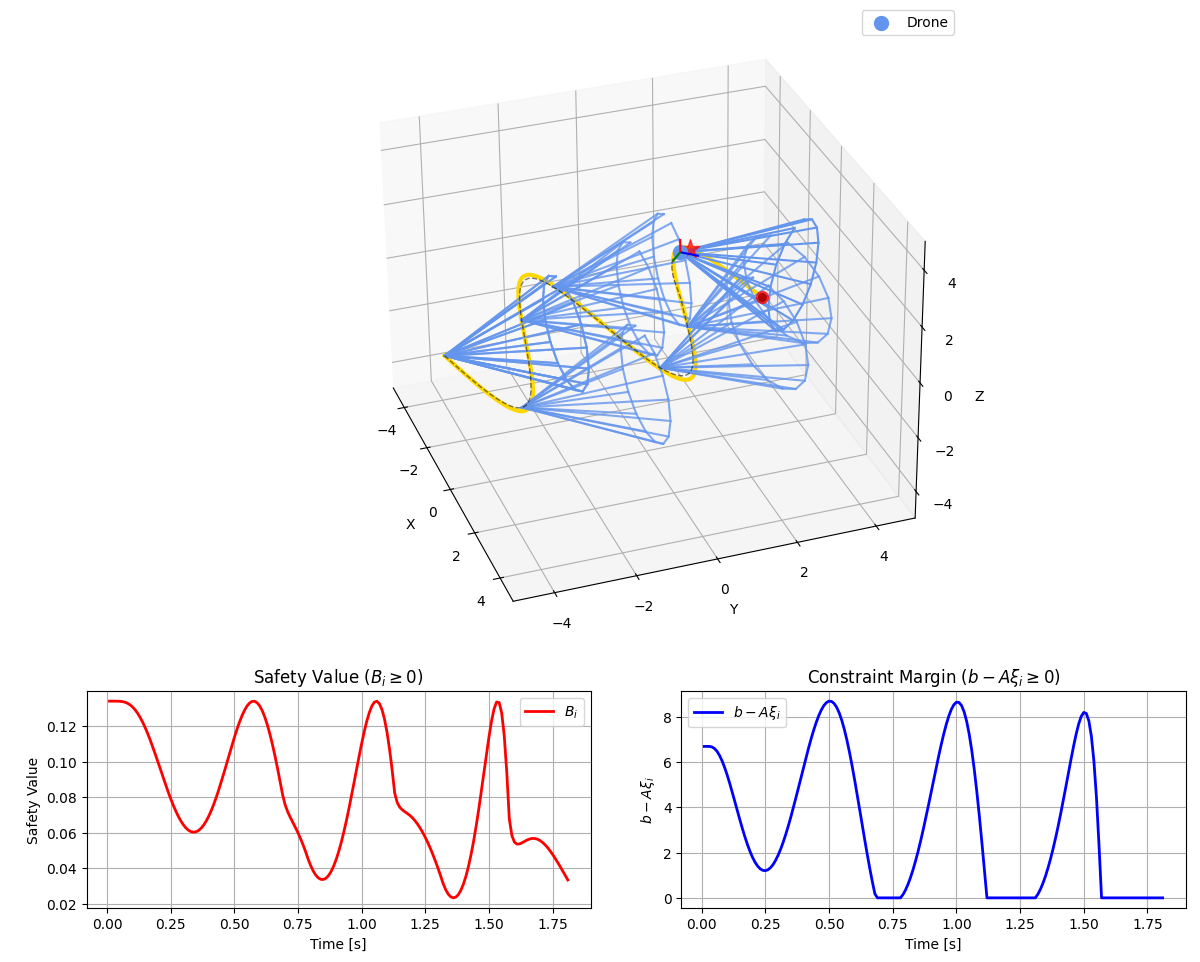
\includegraphics[width=0.6\linewidth]{fig/point_single.png}
\caption{単一特徴点追従におけるエージェントの軌跡と視野錐台}
\label{fig:single_trajectory}
\end{figure}

\subsection{単一エージェントにおける複数特徴点追従のためのCBF}

次に,単一エージェントが複数の特徴点を同時に追従する場合のシミュレーション結果について述べる.表\ref{tab:multi_point_params}に示すパラメータを用いてシミュレーションを実施した.ここで,前節のパラメータに加えて,$q$は\Eqref{eq:multi_safe_set}における確率制約パラメータである.

\begin{table}[htbp]
\centering
\caption{複数特徴点追従シミュレーションのパラメータ}
\label{tab:multi_point_params}
\begin{tabular}{cc}
\hline
変数名 & 値 \\
\hline
$h$ & $0.02$ \\
$\Psi_{\mathcal{F}}$ & $30^{\circ}$ \\
$Q_1$ & $\mathbf{I}_3$ \\
$Q_2$ & $0.0005\times\mathbf{I}_6$ \\
$q$ & $0.5$ \\
$\gamma_0$ & $5.0$ \\
\hline
\end{tabular}
\end{table}

図\ref{fig:multi_trajectory}に複数特徴点追従におけるエージェントの軌跡と視野錐台を示す.単一特徴点追従の場合と同様に,各タイムステップにおいてエージェント$i$が複数の特徴点を視野内に維持しながら追従していることが確認できる.安全制約$B_{i}$の値が常に正の値を保っており,CBFの正不変性が保証されていることがわかる.また,安全制約が減少傾向を示すタイムステップにおいて,制約余裕が零になっていることから,CBFが適切に機能していることが確認できる.

\begin{figure}[htbp]
\centering
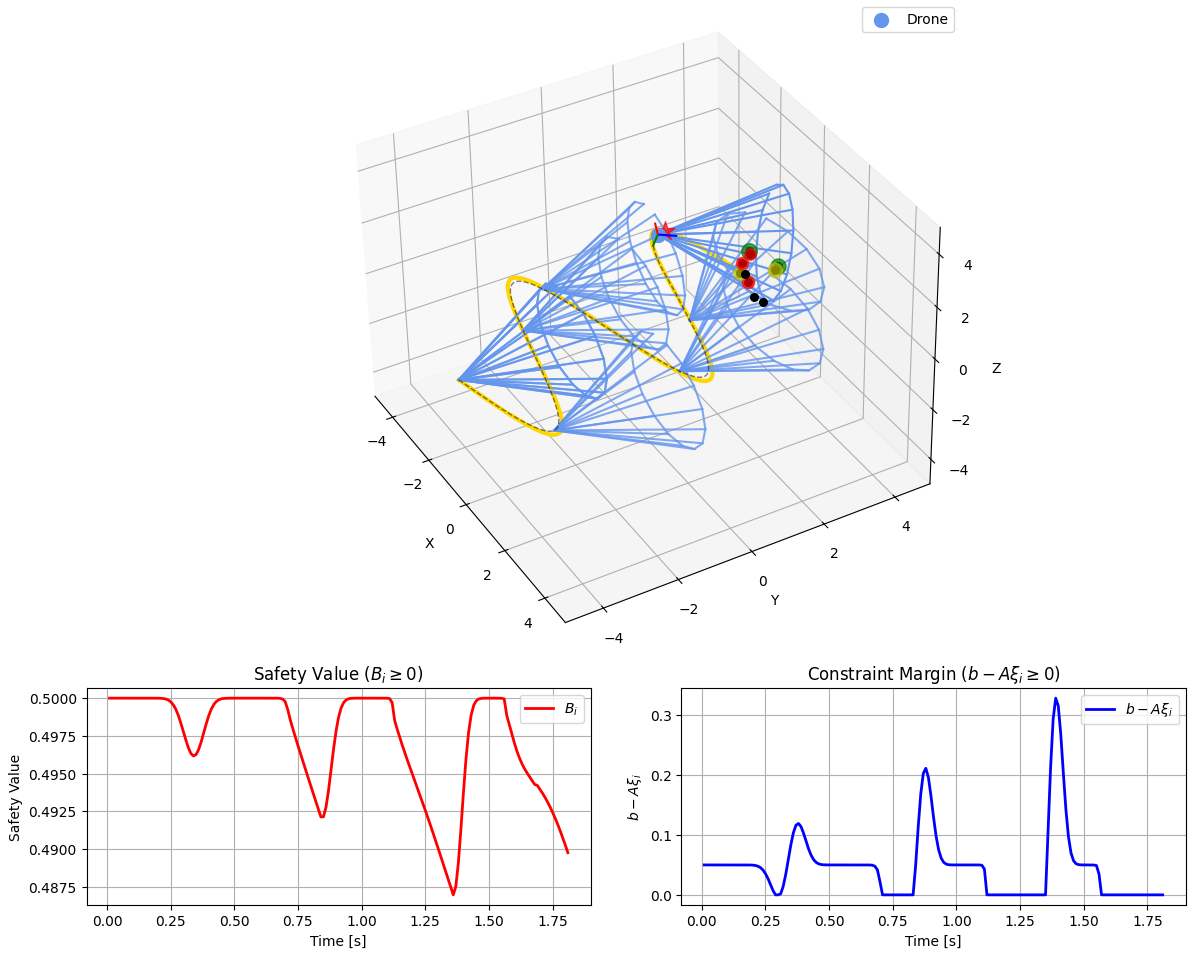
\includegraphics[width=0.6\linewidth]{fig/pcl_single.png}
\caption{複数特徴点追従におけるエージェントの軌跡と視野錐台}
\label{fig:multi_trajectory}
\end{figure}

\subsection{複数エージェントにおける複数特徴点追従のための集中型CBF}

続いて,複数エージェントが複数の特徴点を共有視野内に維持しながら追従する場合の集中型制御によるシミュレーション結果について述べる.表\ref{tab:centralized_params}に示すパラメータを用いてシミュレーションを実施した.

\begin{table}[htbp]
\centering
\caption{集中型制御シミュレーションのパラメータ}
\label{tab:centralized_params}
\begin{tabular}{cc}
\hline
変数名 & 値 \\
\hline
$h$ & $0.02$ \\
$\Psi_{\mathcal{F}}$ & $30^{\circ}$ \\
$Q_1$ & $\mathbf{I}_3$ \\
$Q_2$ & $0.0005\times\mathbf{I}_6$ \\
$q$ & $0.3$ \\
$\gamma_0$ & $0.1$ \\
\hline
\end{tabular}
\end{table}

図\ref{fig:centralized_trajectory}に集中型制御における複数エージェントの軌跡と視野錐台を示す.各タイムステップにおいて,エージェント$i$とエージェント$j$が共有特徴点を視野内に維持しながら協調して動作していることが確認できる.安全制約$B_{ij}$の値が常に正の値を保っており,CBFの正不変性が保証されていることがわかる.また,安全制約が減少傾向を示すタイムステップにおいて,制約余裕が零になっていることから,CBFが適切に機能していることが確認できる.

\begin{figure}[htbp]
\centering
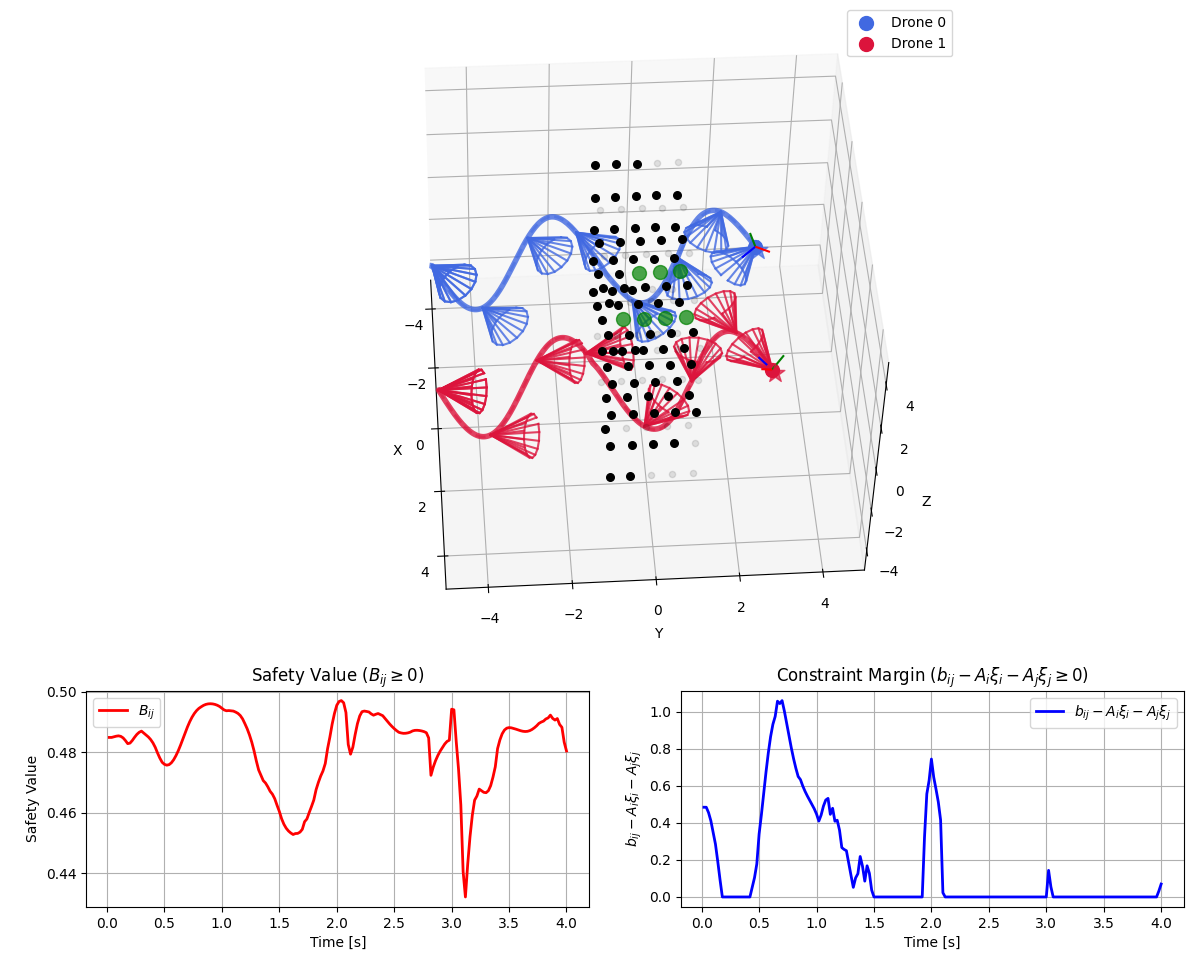
\includegraphics[width=0.6\linewidth]{fig/pcl_multi_centric.png}
\caption{複数特徴点追従における複数エージェントの軌跡と視野錐台}
\label{fig:centralized_trajectory}
\end{figure}

\subsection{複数エージェントにおける複数特徴点追従のための分散型CBF}

最後に,複数エージェントが複数の特徴点を共有視野内に維持しながら追従する場合の分散型制御によるシミュレーション結果について述べる.表\ref{tab:distributed_params}に示すパラメータを用いてシミュレーションを実施した.ここで,前節のパラメータに加えて,$c$は\Eqref{eq:pdmm_algorithm}における分散最適化のペナルティパラメータである.

\begin{table}[htbp]
\centering
\caption{分散型制御シミュレーションのパラメータ}
\label{tab:distributed_params}
\begin{tabular}{cc}
\hline
変数名 & 値 \\
\hline
$h$ & $0.02$ \\
$\Psi_{\mathcal{F}}$ & $30^{\circ}$ \\
$Q_1$ & $0.5\times \mathbf{I}_3$ \\
$Q_2$ & $0.00001\times\mathbf{I}_6$ \\
$q$ & $0.3$ \\
$\gamma_0$ & $0.1$ \\
$c$ & $1.0$ \\
\hline
\end{tabular}
\end{table}

図\ref{fig:distributed_trajectory}に分散型制御における複数エージェントの軌跡と視野錐台を示す.各タイムステップにおいて,エージェント$i$とエージェント$j$が共有特徴点を視野内に維持しながら協調して動作していることが確認できる.分散型最適化においては,元の制約式を直接解くことは不可能であるが,エージェント$i$が評価することのできる$A_i\xi_i-\frac{1}{2}b_{ij}$およびエージェント$j$の$A_j\xi_j-\frac{1}{2}b_{ij}$の和が適切に制約を満たしていることがわかる.これにより,各エージェントが局所的な情報のみを用いて,大域的な安全制約を満たす制御入力を生成できていることが確認できる.

\begin{figure}[htbp]
\centering
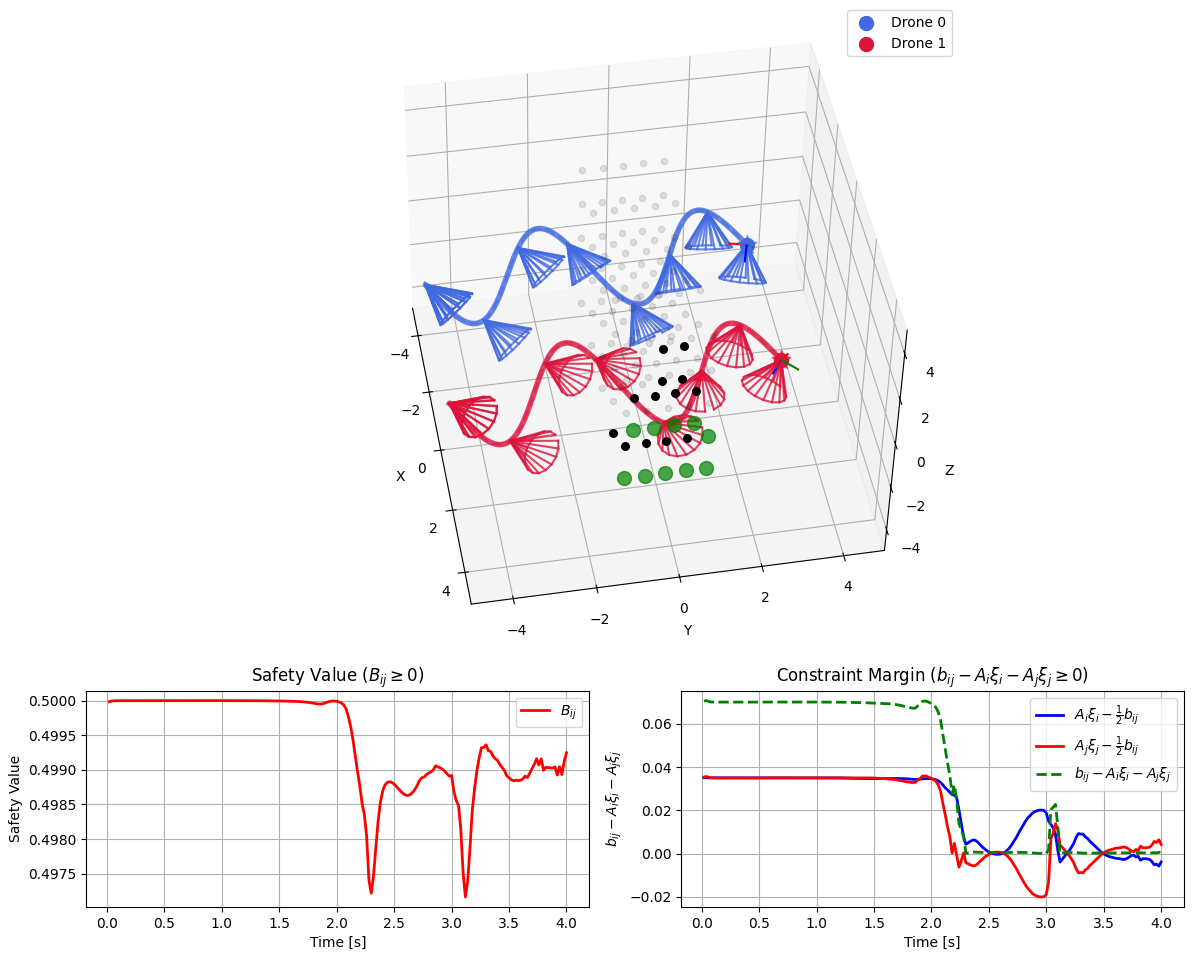
\includegraphics[width=0.6\linewidth]{fig/pcl_multi_distrib.png}
\caption{分散実装におけるエージェントの軌跡と視野錐台}
\label{fig:distributed_trajectory}
\end{figure}

以上のシミュレーション結果から,提案手法が単一エージェントおよび複数エージェントの両方において,特徴点を視野内に維持しながら追従するという制約を満たす制御入力を生成できることが確認された.特に,分散型実装においても,各エージェントが局所的な情報のみを用いて,大域的な安全制約を満たす制御入力を生成できることが示された.

\section{結論及び展望}

本研究では,SE(3)上における協調自己位置推定のための視野共有を保証する分散型CBFを提案した.特に,複数のエージェントが共通の特徴点を観測することで,自己位置推定の精度を向上させるための制御手法を開発した.以下に今後の展望について述べる.

\subsection{確率関数の設計によるアクティブパーセプション}

視野共有を保証するCBFにおいては,特徴点$q_l$がエージェント$i$の視野内にあるかどうかを表す関数$\Psi_{i}^l$が重要な役割を果たす.\Eqref{eq:single_fov_condition}で示したように,この関数は以下のように定義される:
\begin{equation}
\begin{aligned}
\Psi_{i}^l = \left\{ \begin{array}{ll}
0 & \mathrm{if} \quad  \beta_l^{\top}(p_i)R_ie_c-\cos\Psi_{\mathcal{F}} < 0\\
1 & \mathrm{if}  \quad  \beta_l^{\top}(p_i)R_ie_c-\cos\Psi_{\mathcal{F}} \geq 0
\end{array} \right.
\end{aligned}
\label{eq:psi_function}
\end{equation}

しかし,この関数は微分不可能であるため,CBFの設計において問題となる.そこで本研究では,特徴点$q_l \in \mathcal{L}$によってエージェント$i$における推定が成り立っている確率を表す関数$\phi_{i}^l$を導入した:
\begin{equation}
\begin{aligned}
\phi_{i}^l= P(p_i,R_i,q^l)
\end{aligned}
\label{eq:phi_function}
\end{equation}

本研究では,簡単のために以下の確率関数を使用した:
\begin{equation}
\begin{aligned}
P_i^l &= \frac{\beta_l^\top(p_i) R_i e_c -\cos\Psi_{\mathcal{F}} }{1-\cos\Psi_{\mathcal{F}}}
\end{aligned}
\label{eq:p_function}
\end{equation}
ここで,$\beta_l$はエージェント$i$から特徴点$q_l$への単位方向ベクトル,$R_i$はエージェント$i$の姿勢行列,$e_c$はカメラの光軸方向を表す単位ベクトル,$\Psi_{\mathcal{F}}$はカメラの視野角の半分である.この確率関数は,特徴点がカメラの光軸に近いほど高い値を取り,視野角の境界では0になるという性質を持つ.

\subsection{自己位置推定における確率関数の理論的裏付け}

$P^l_i$が$(p_i, R_i)\in \mathrm{SE(3)}$について微分可能であれば,任意の確率関数を設計可能である.本研究では,自己位置推定における理論的な裏付けに基づいた確率関数の設計について検討した.

各エージェント$i \in \mathcal{A}$に対して,観測モデルは以下のように表される:
\begin{equation}
\begin{aligned}
\tilde{p}_i = \pi_i(q_l) + w_i
\end{aligned}
\label{eq:observation_model}
\end{equation}
ここで,$\pi_i(q_l)$はエージェント$i$における$q_l$の非線形な投影関数であり,$w_i$は白色ノイズである.通常,$w_i$は独立同分布の正規分布$w_i \sim \mathcal{N}(0, \sigma_i^2 I)$と仮定される.

最尤推定量$\hat{q}_l$は,以下の最適化問題の解として求められる:
\begin{equation}
\begin{aligned}
\hat{q}_l = \operatorname*{arg\,min}_{q_l} \sum_i \| \tilde{p}_i - \pi_i(q_l) \|^2_{\Sigma_i^{-1}}
\end{aligned}
\label{eq:mle}
\end{equation}
ここで,$\Sigma_i$は$w_i$の共分散行列である.

投影関数$\pi_i(q_l)$は一般に非線形であるため,解析的に誤差伝搬や不確かさを評価するには,$q_l$の推定値の周りで一階テイラー展開を用いる.任意の推定点$q_0^l$周りで:
\begin{equation}
\begin{aligned}
\pi_i(q_l) \approx \pi_i(q_0^l) + J_i (q_l - q_0^l)
\end{aligned}
\label{eq:taylor_expansion}
\end{equation}
と近似する.ここで,$J_i = \frac{\partial \pi_i}{\partial q_l} \Big|_{q_l=q_0^l}$はエージェント$i$における投影関数のヤコビアンである.

最尤推定問題において,推定値の下界としてのCramer-Rao Lower Bound (CRLB)は,フィッシャー情報行列$\mathbf{I}(q_l)$を用いて記述される:
\begin{equation}
\begin{aligned}
\mathbf{I}(q_l) = \sum_i J_i^T \Sigma_i^{-1} J_i
\end{aligned}
\label{eq:fim}
\end{equation}

\begin{dfn}[Cramer--Rao Lower Bound]
確率変数 $\mathbf y\in\mathbb R^{m}$ が母数 $\boldsymbol\theta\in\mathbb R^{p}$ に依存し,
確率密度 $p(\mathbf y;\boldsymbol\theta)$ をもつとする.  
$\hat{\boldsymbol\theta}(\mathbf y)$ が $\boldsymbol\theta$ の不偏推定量
(すなわち $\mathbb E[\hat{\boldsymbol\theta}]=\boldsymbol\theta$)であるとき,
その共分散行列は
\[
    \operatorname{Cov}(\hat{\boldsymbol\theta})
    \;\succeq\;
    \mathbf I(\boldsymbol\theta)^{-1},
    \qquad
    \mathbf I(\boldsymbol\theta)
    :=\mathbb E\!\left[
        \left(\nabla_{\!\boldsymbol\theta}\!\log p(\mathbf y;\boldsymbol\theta)\right)
        \,\left(\nabla_{\!\boldsymbol\theta}\!\log p(\mathbf y;\boldsymbol\theta)\right)^{\!\top}
    \right]
\]
で下から抑えられる.  
ここで $\mathbf I(\boldsymbol\theta)$ は
フィッシャー情報行列と呼ばれる行列である.
この不等式をCramer--Rao Lower Boundと呼ぶ.
\end{dfn}

観測モデル\eqref{eq:observation_model}の下で,パラメータ$q_l$に関する対数尤度関数を
\begin{equation}
\begin{aligned}
\ell(q_l)
&= -\frac{1}{2}\sum_{i=1}^m
(\tilde p_i - \pi_i(q_l))^\top \Sigma_i^{-1}(\tilde p_i - \pi_i(q_l)) + C
\label{eq:loglikelihood_expanded}
\end{aligned}
\end{equation}
と書く。ここで$C$は$q_l$に依存しない定数である。

まず,$\ell(q_l)$の勾配(一次微分)を計算すると
\begin{equation}
\begin{aligned}
\nabla_{q_l}\ell(q_l)
&= \sum_{i=1}^m
\frac{\partial \pi_i}{\partial q_l}^\top
\Sigma_i^{-1}(\tilde p_i - \pi_i(q_l))
= \sum_{i=1}^m J_i^\top \Sigma_i^{-1}(\tilde p_i - \pi_i(q_l)),
\end{aligned}
\label{eq:grad_loglikelihood}
\end{equation}
となる。

次に,二次微分(ヘッセ行列)を取ると
\begin{equation}
\begin{aligned}
\nabla^2_{q_l}\ell(q_l)
&= -\sum_{i=1}^m
J_i^\top \Sigma_i^{-1} J_i
\;+\;\underbrace{\sum_{i=1}^m
(\tilde p_i - \pi_i(q_l))^\top
\Sigma_i^{-1}
\frac{\partial^2 \pi_i}{\partial q_l^2}}_{A(q_l)}.
\end{aligned}
\label{eq:hessian_loglikelihood}
\end{equation}
ガウス雑音の性質より,期待値を取ると残差項$(\tilde p_i - \pi_i)$の平均は零になるため
\begin{equation}
\begin{aligned}
-\mathbb{E}\bigl[\nabla^2_{q_l}\ell(q_l)\bigr]
&= \sum_{i=1}^m J_i^\top \Sigma_i^{-1} J_i.
\end{aligned}
\label{eq:FIM_derivation}
\end{equation}

以上より任意の不偏推定量$\hat{q}_l$の共分散行列は次の下界を満たす:
\begin{equation}
\begin{aligned}
\operatorname{Cov}(\hat{q}_l) \ge \mathbf{I}(q_l)^{-1} = \left( \sum_i J_i^T \Sigma_i^{-1} J_i \right)^{-1}
\end{aligned}
\label{eq:crlb}
\end{equation}

特に,各エージェントのノイズが等方性(すべて$\Sigma_i = \sigma^2 I$とする場合),上式は以下のように簡略化される:
\begin{equation}
\begin{aligned}
\operatorname{Cov}(\hat{q}_l) \ge \sigma^2 \left( \sum_i J_i^T J_i \right)^{-1}
\end{aligned}
\label{eq:crlb_isotropic}
\end{equation}

この式から,エージェント数が増えることにより各々の寄与が積み重なり,結果として推定の不確かさが低下する傾向が明確となる.
各エージェントについて,対象$q_l$の投影に関する解析的なヤコビアンは以下のように記述できる:
\begin{equation}
\begin{aligned}
J_i = \frac{f}{d_i}\,P_{\beta_i}, \quad d_i = \|q_l-p_i\|, \quad P_{\beta_i} = I - \beta_i\,\beta_i^\top
\end{aligned}
\label{eq:jacobian}
\end{equation}
ここで,$f$は焦点距離,$d_i$は対象とエージェント$i$との距離,$\beta_i = \frac{q_l-p_i}{d_i}$はエージェント$i$におけるbearing,$P_{\beta_i}$は$\beta_i$に沿った成分を取り除く射影行列である.

エージェント$i$と$j$からのフィッシャー情報行列は以下のように計算できる:
\begin{equation}
\begin{aligned}
I_i &= J_i^\top J_i = \frac{f^2}{d_i^2}\,P_{\beta_i} \\
I_j &= J_j^\top J_j = \frac{f^2}{d_j^2}\,P_{\beta_j}
\end{aligned}
\label{eq:fim_individual}
\end{equation}

したがって,2台のカメラからの合成情報は以下のようになる:
\begin{equation}
\begin{aligned}
I_{\text{total}} = J_i^\top J_i + J_j^\top J_j = \frac{f^2}{d_i^2}\,P_{\beta_i} + \frac{f^2}{d_j^2}\,P_{\beta_j}
\end{aligned}
\label{eq:fim_total}
\end{equation}

CRLBにより,無偏推定量$\hat{q}_l$の共分散行列は以下の下界を満たす:
\begin{equation}
\begin{aligned}
\operatorname{Cov}(q_l) \ge \sigma^2\,\frac{1}{f^2}\,\left[\frac{P_{\beta_i}}{d_i^2} + \frac{P_{\beta_j}}{d_j^2}\right]^{-1}
\end{aligned}
\label{eq:crlb_two_cameras}
\end{equation}

上記の理論的考察に基づき,新しい確率関数を以下のように設計することができる:
\begin{equation}
\begin{aligned}
P_i^l &= \exp\left(-\frac{\sigma^2}{f^2}\,\mathrm{tr}\left[\frac{P_{\beta_i}}{d_i^2} + \frac{P_{\beta_j}}{d_j^2}\right]^{-1}\right)
\end{aligned}
\label{eq:new_probability_function}
\end{equation}

\Figref{fig:drone_setup}に示すようにエージェントを設置した場合,エージェント$i$と$j$の視野錐台が接する断面における確率関数の値をそれぞれ\Figref{fig:potential_comparison}に示す

\begin{figure}[H]
    \centering
    \begin{subfigure}[b]{0.45\linewidth}
        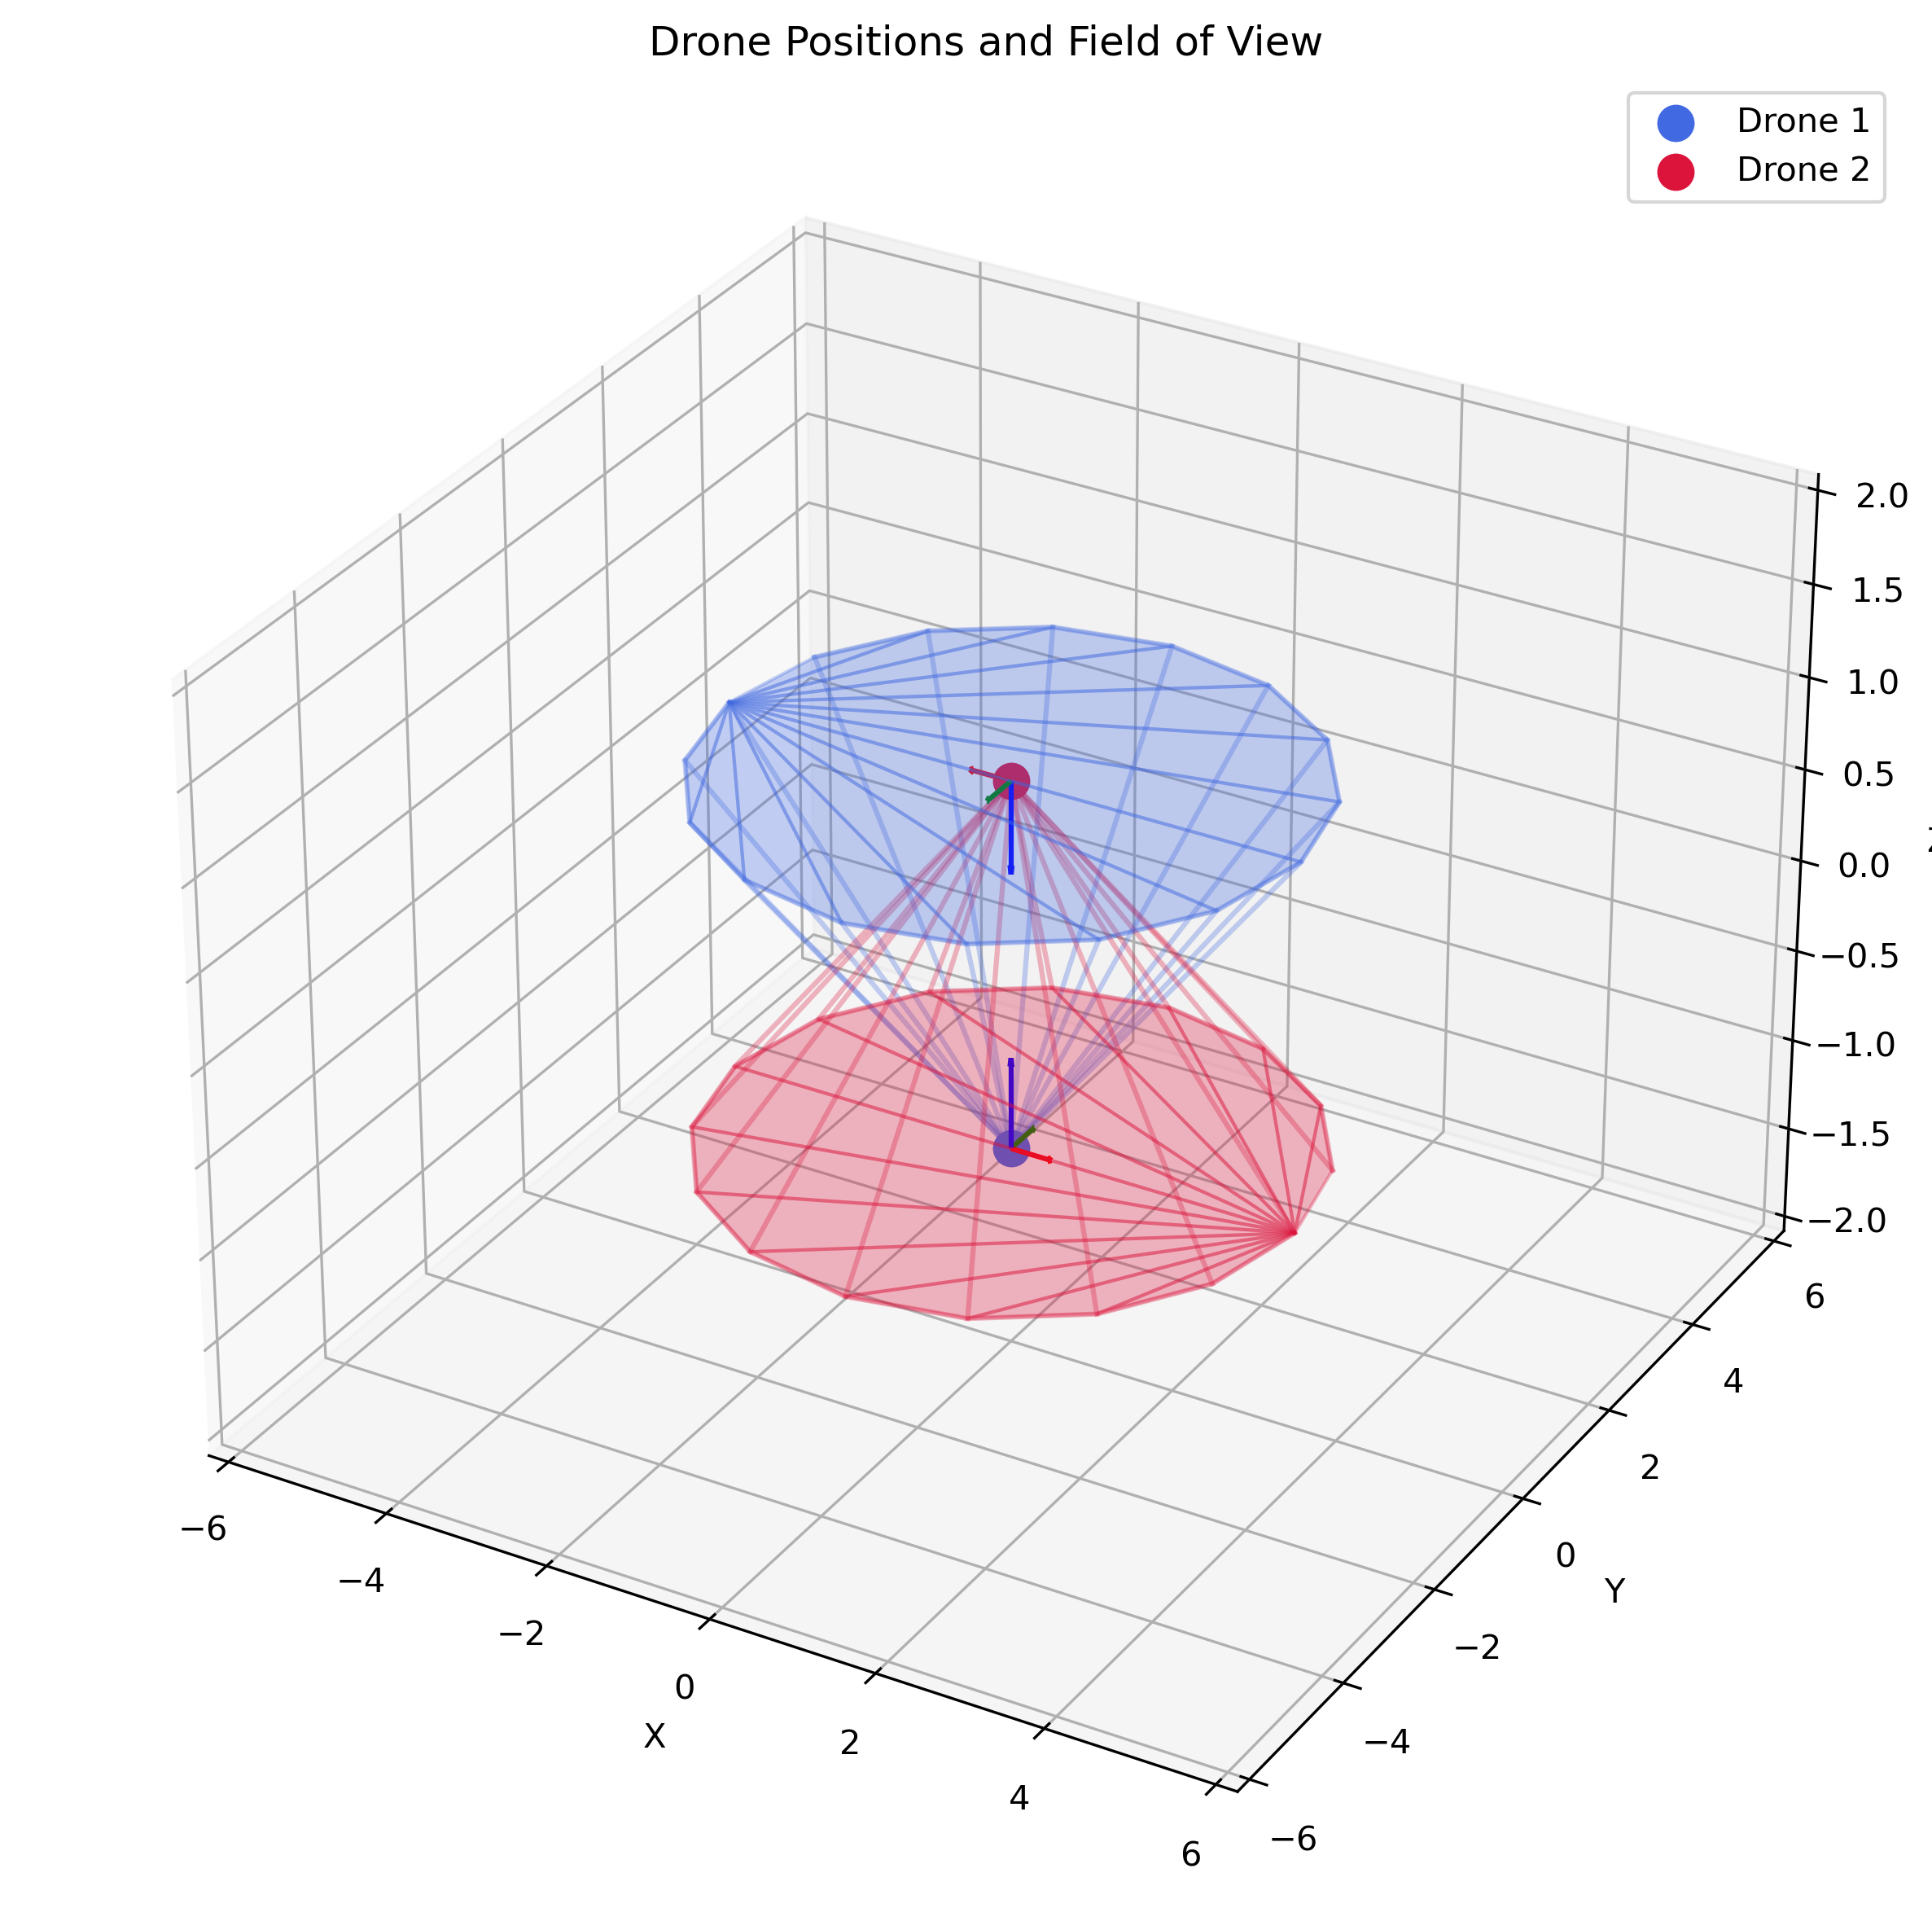
\includegraphics[width=\linewidth]{fig/drone_setup.png}
        \caption{エージェントの設置例}
        \label{fig:drone_setup}
    \end{subfigure}
    \hfill
    \begin{subfigure}[b]{0.45\linewidth}
        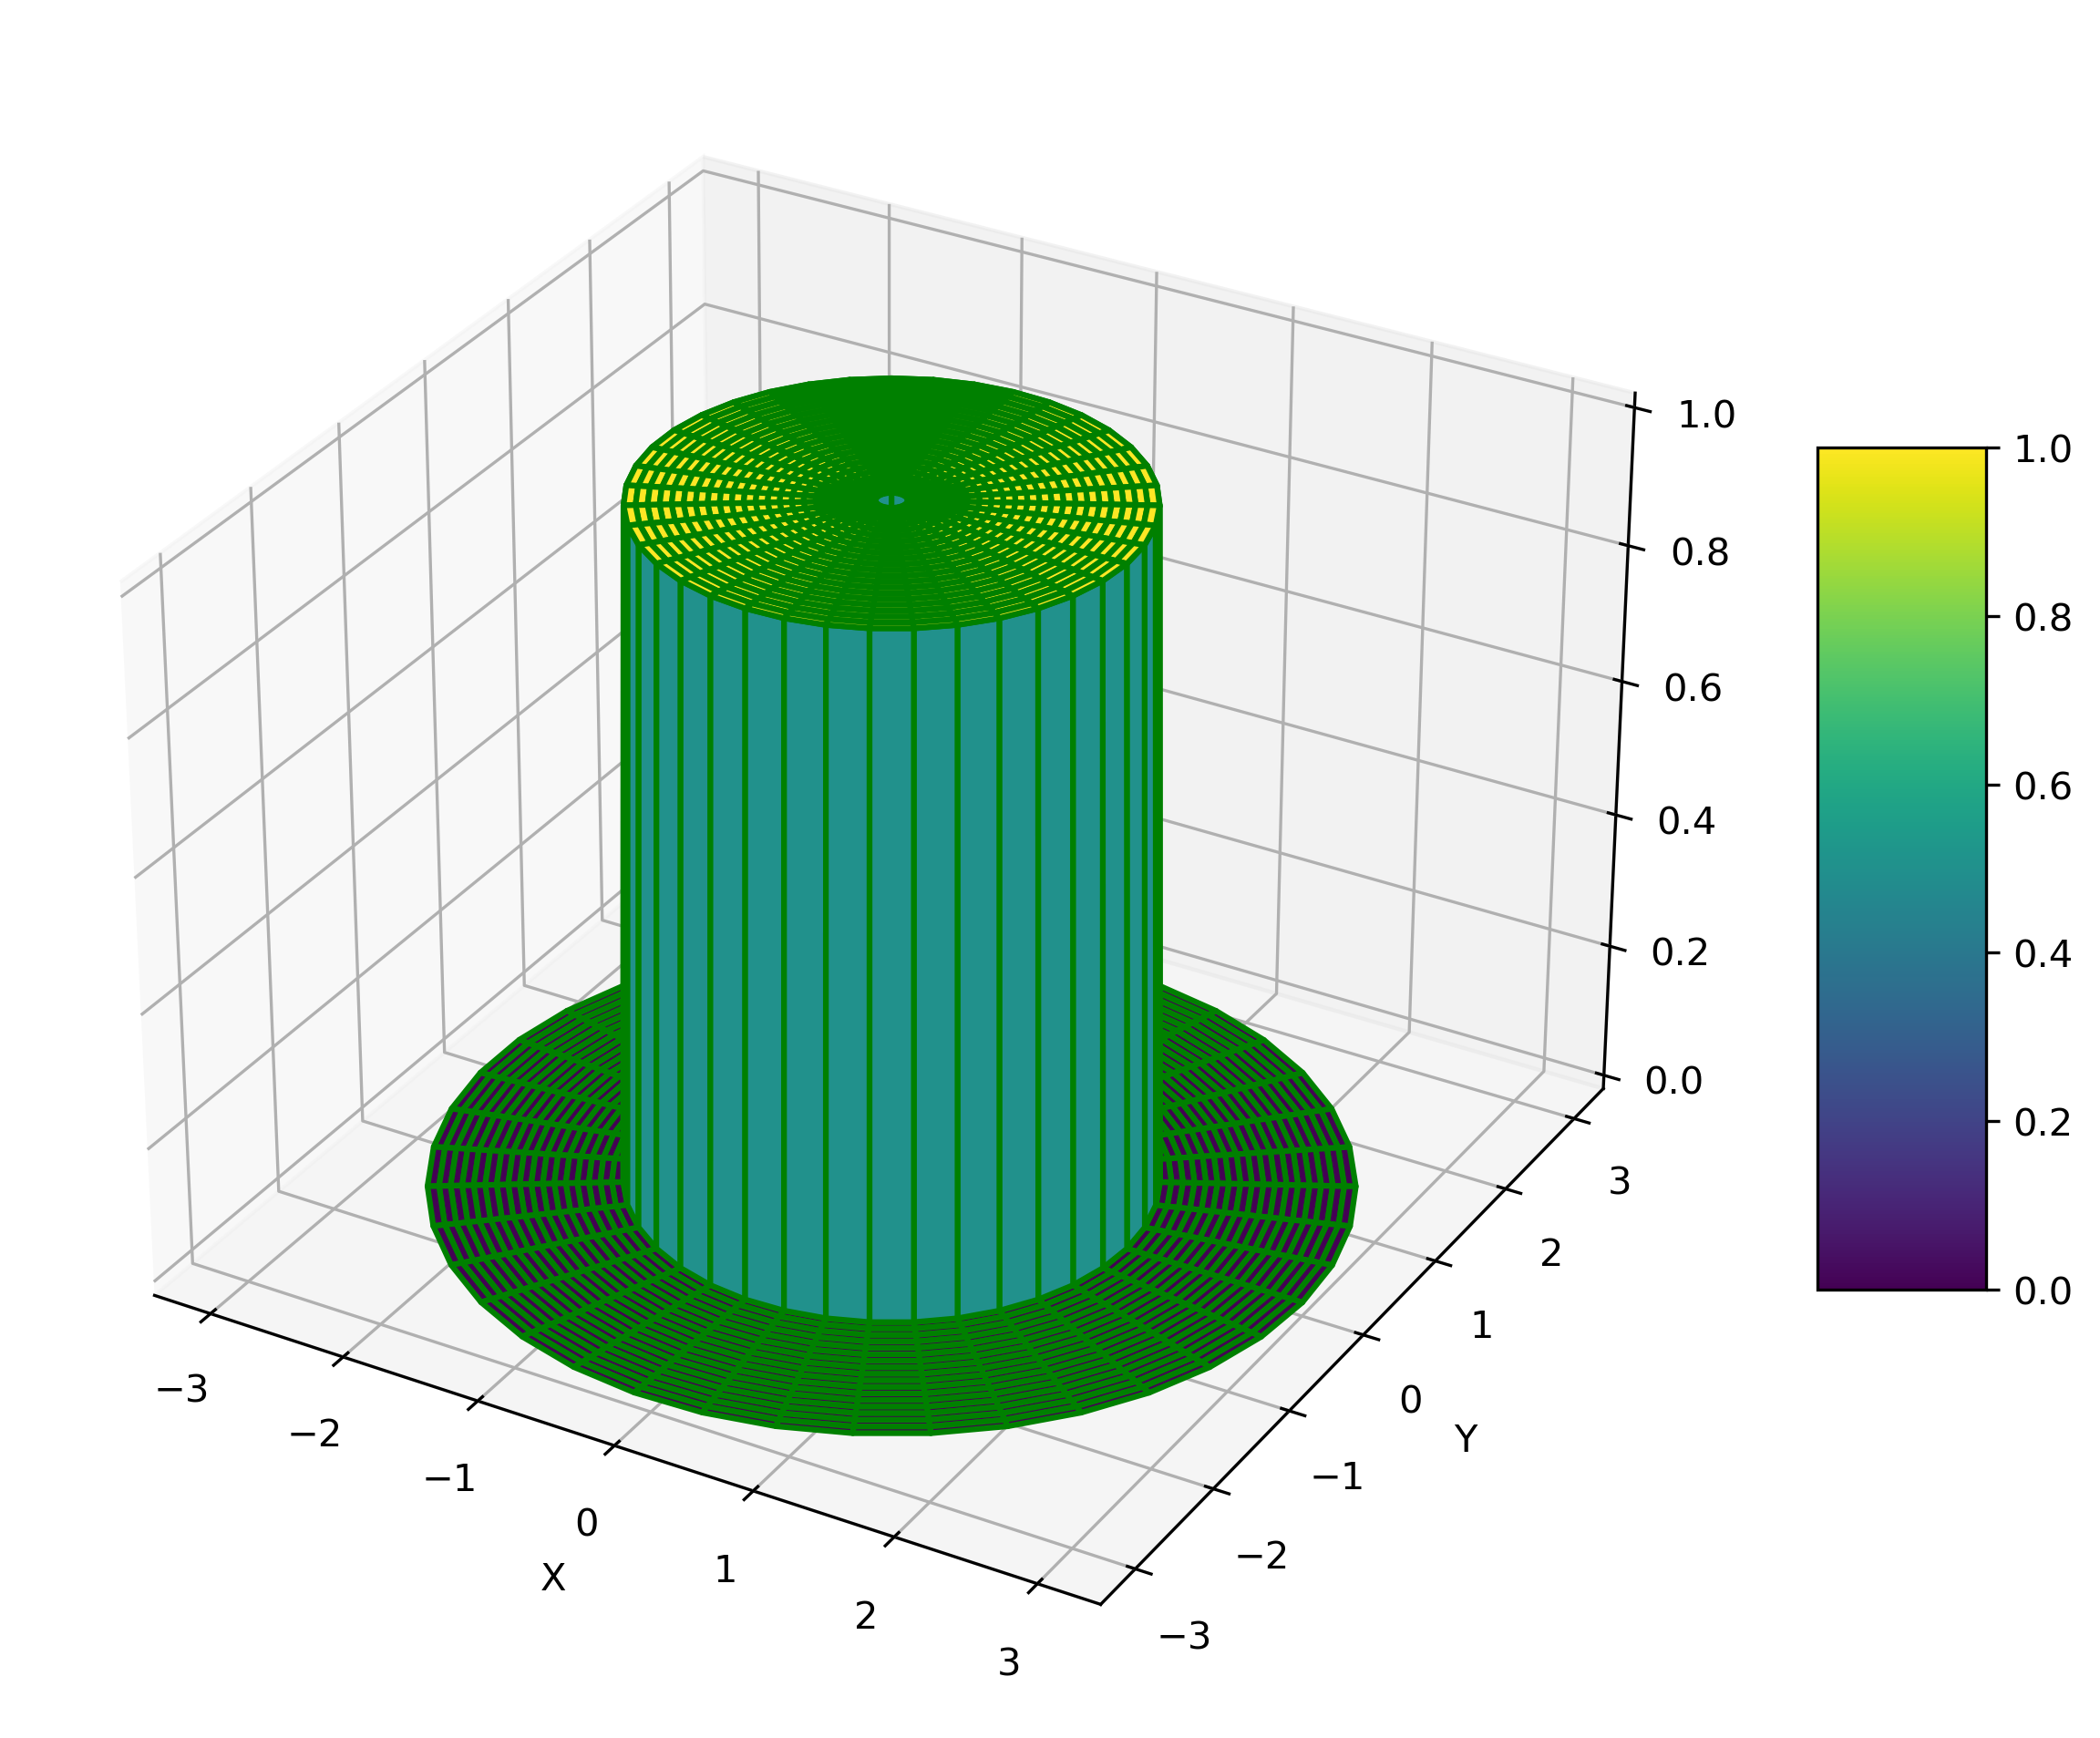
\includegraphics[width=\linewidth]{fig/psi_function_potential.png}
        \caption{$\Psi_{i}^l$関数のポテンシャル\Eqref{eq:psi_function}}
        \label{fig:psi_function_potential}
    \end{subfigure}
    
    \vspace{0.5cm}
    \begin{subfigure}[b]{0.45\linewidth}
        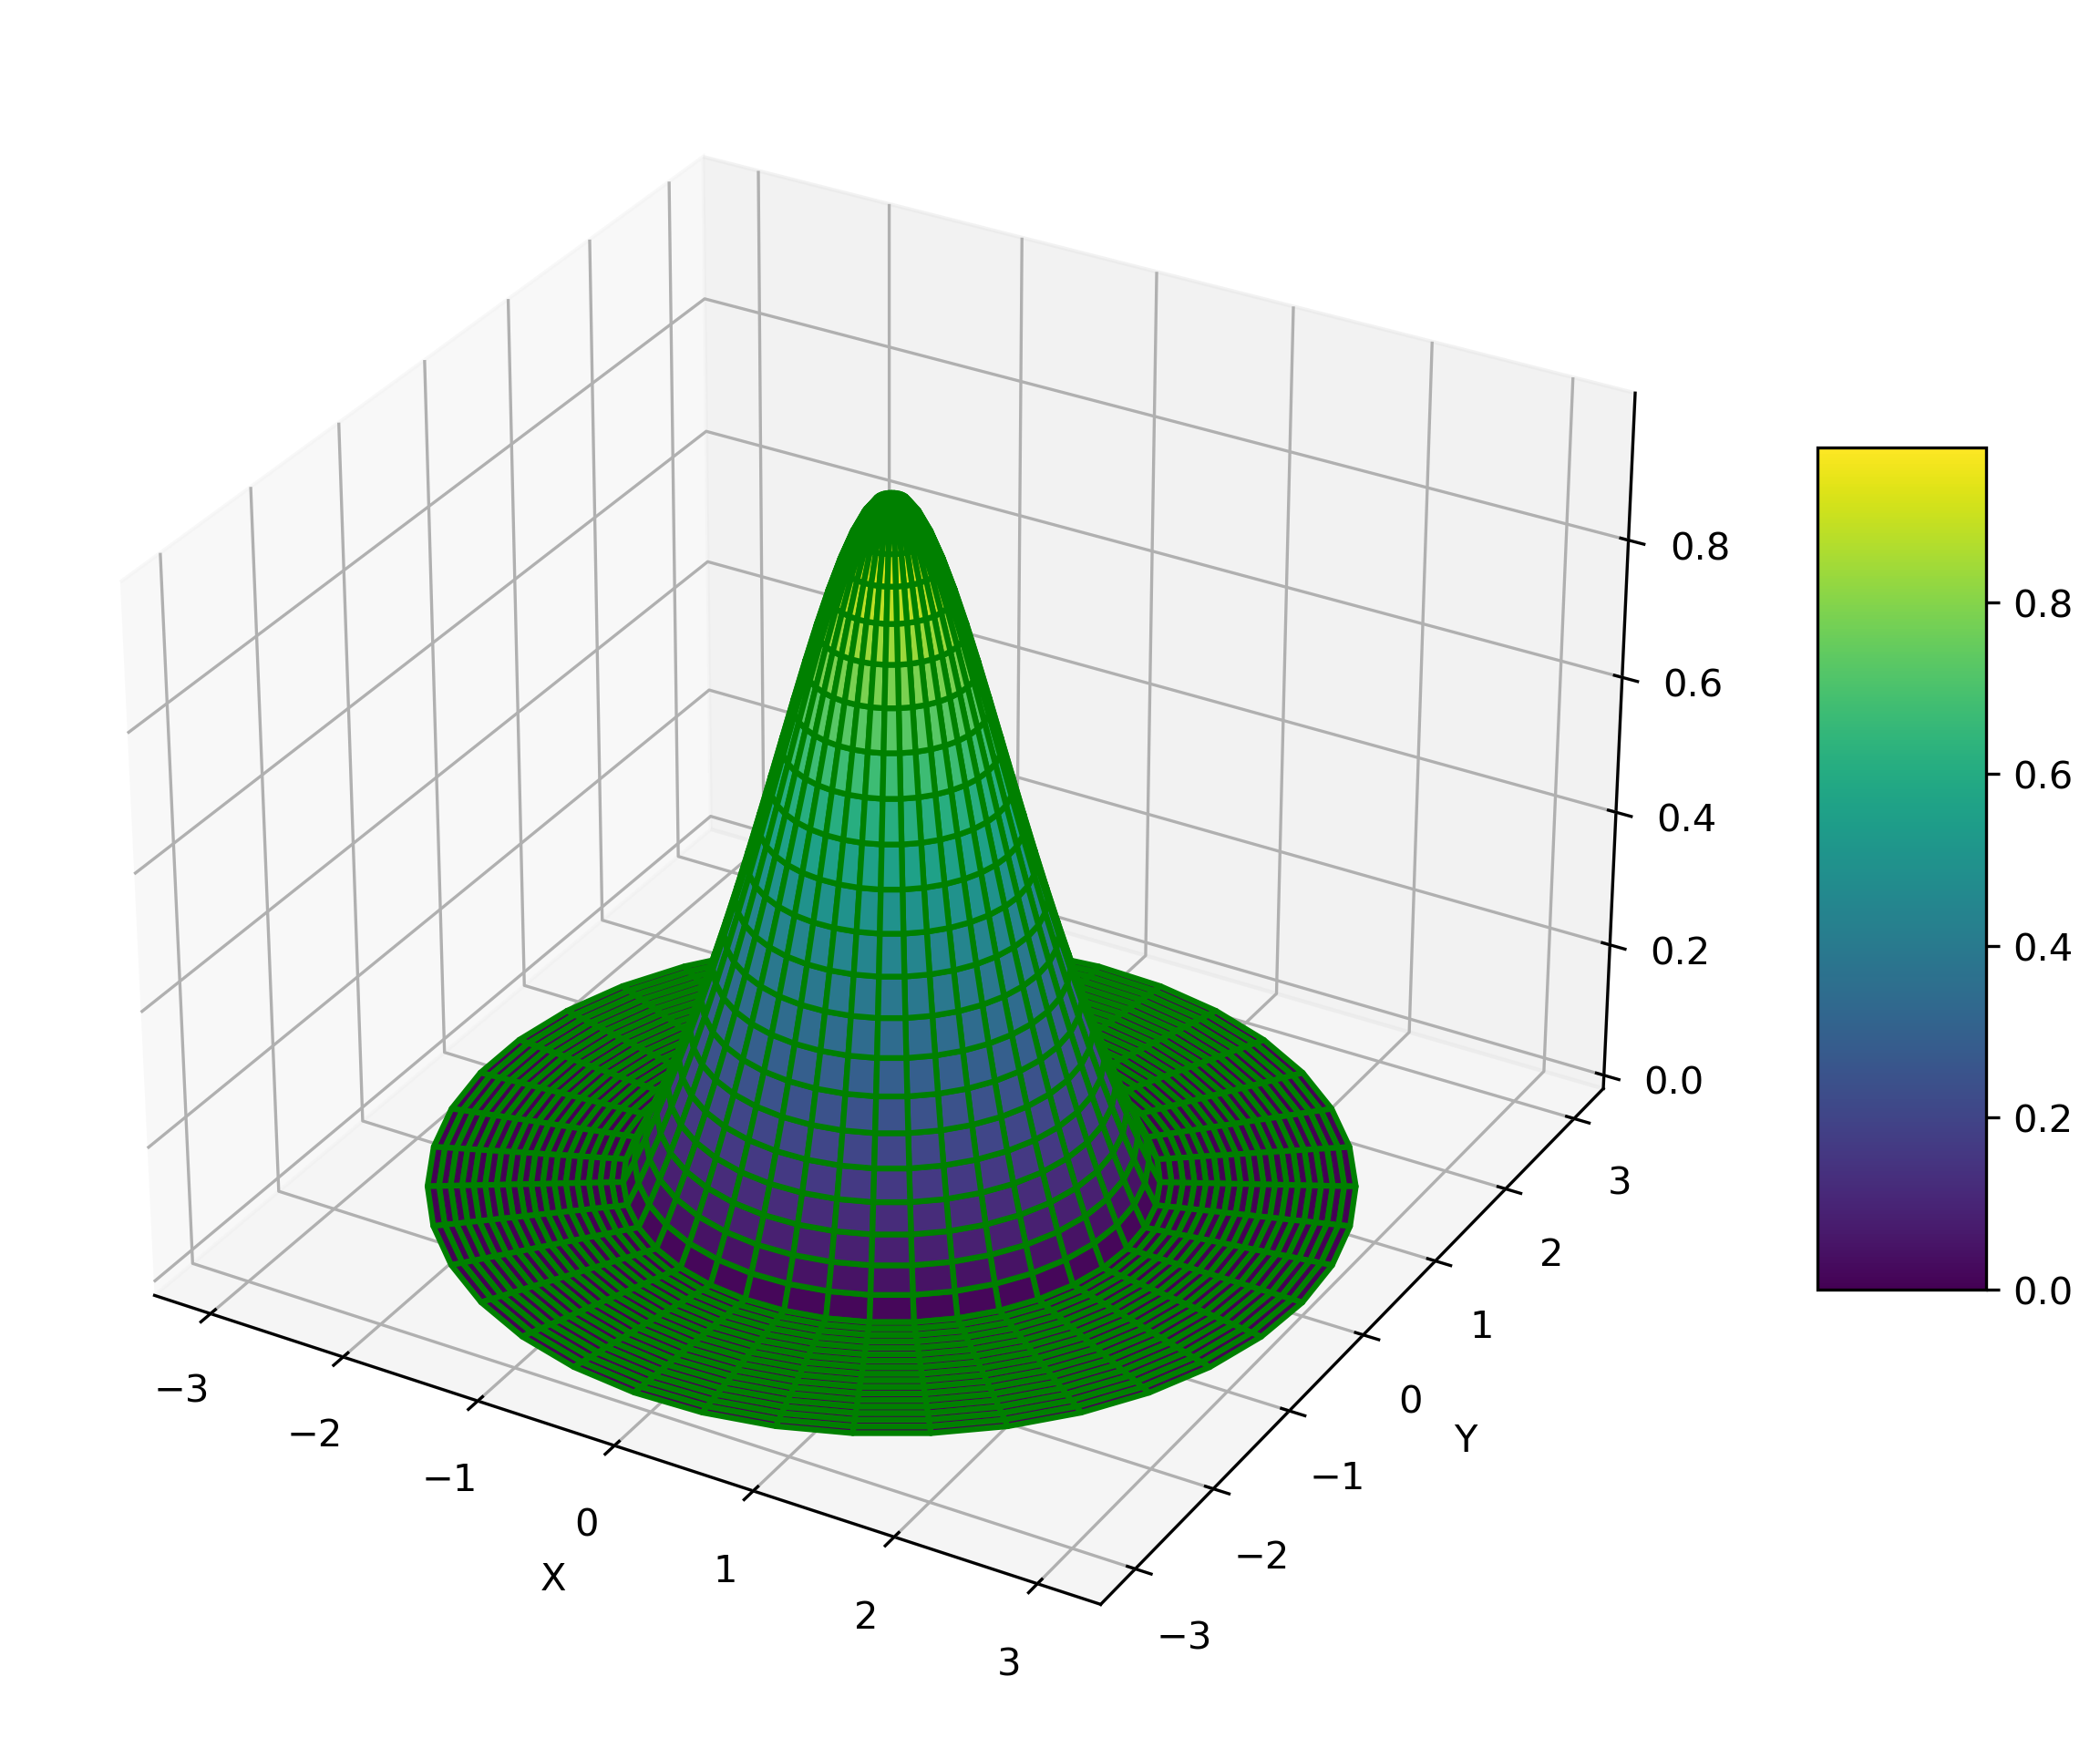
\includegraphics[width=\linewidth]{fig/p_function_potential.png}
        \caption{$P_i^l$関数のポテンシャル\Eqref{eq:new_probability_function}}
        \label{fig:p_function_potential}
    \end{subfigure}
    \hfill
    \begin{subfigure}[b]{0.45\linewidth}
        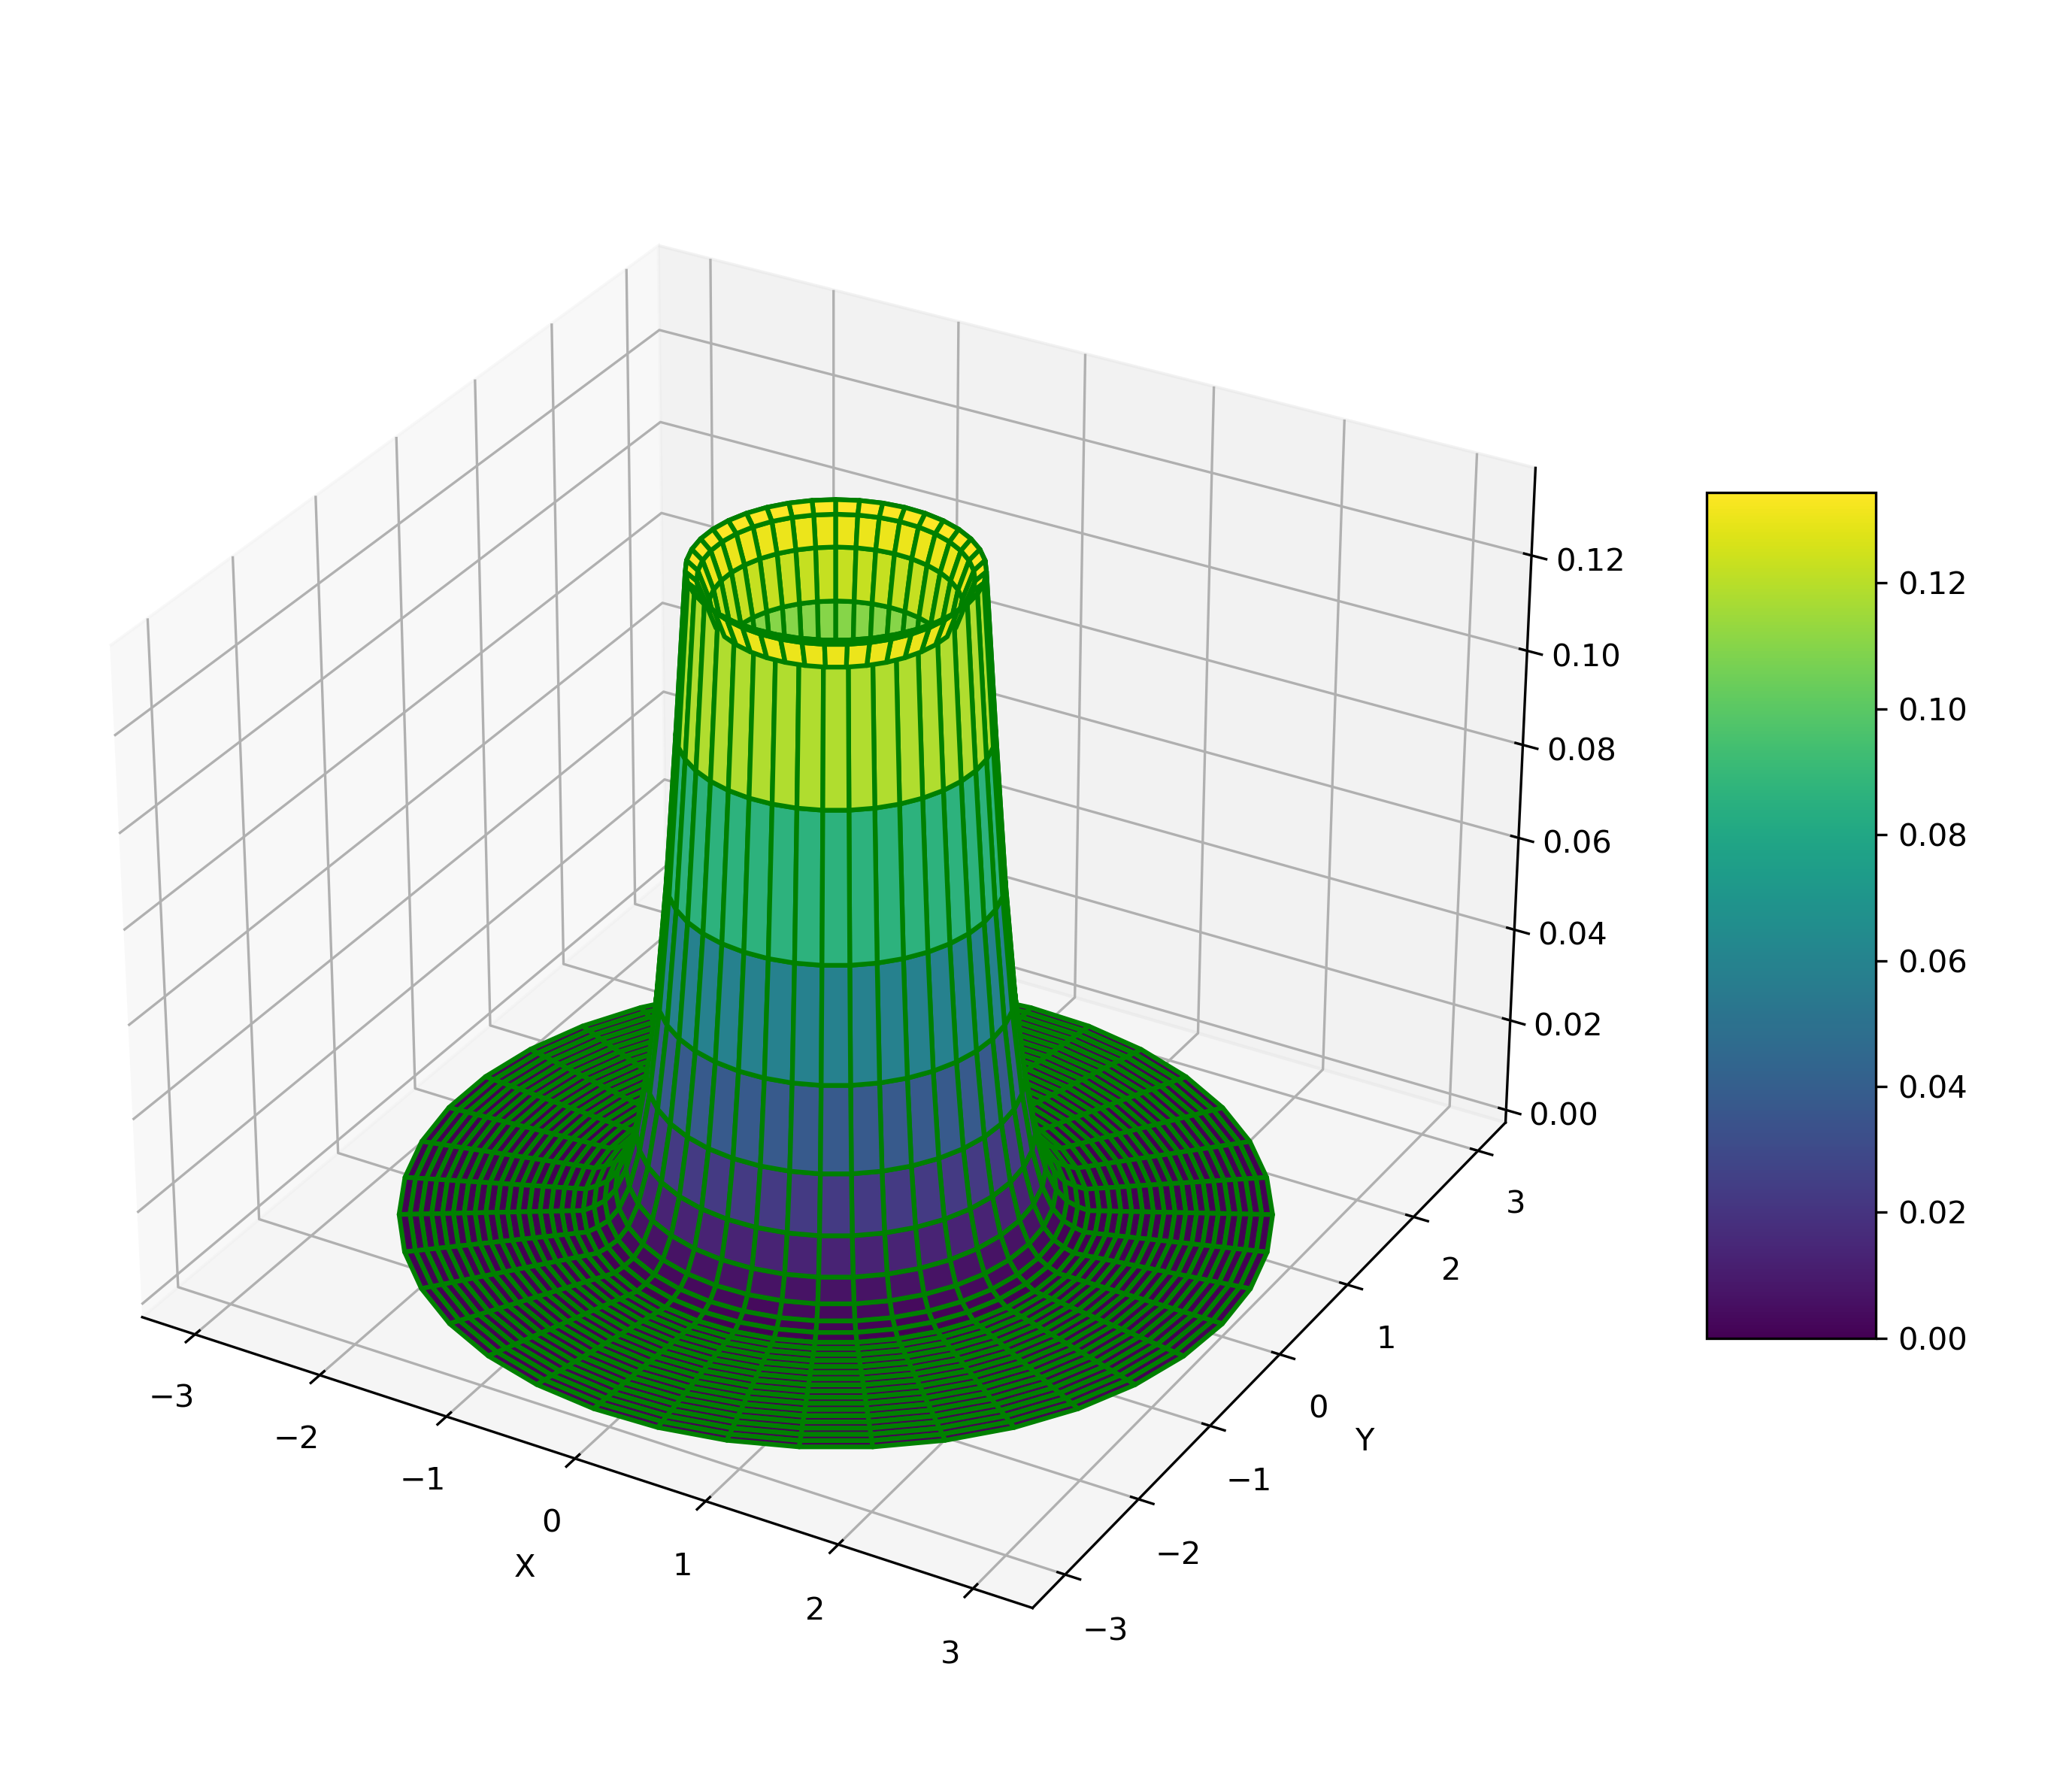
\includegraphics[width=\linewidth]{fig/covariance_function_potential.png}
        \caption{CRLB関数のポテンシャル\Eqref{eq:new_probability_function}}
        \label{fig:covariance_function_potential}
    \end{subfigure}
    \caption{確率関数のポテンシャル}
    \label{fig:potential_comparison}
\end{figure}

また,上記の検討から,\Eqref{eq:new_probability_function}によってCBFを設計する場合,\Figref{fig:CRLB}に示すように,CBFはクラメール・ラオの下限を上から抑える関数として機能することがわかる.クラメール・ラオの下限は最尤推定における最適化限界として働くため,理想的な推定アルゴリズムの元では,視野共有を保証するCBFは自己位置推定を行うためのアクティブパーセプションとして捉えることができる.
\begin{figure}[H]
    \centering
    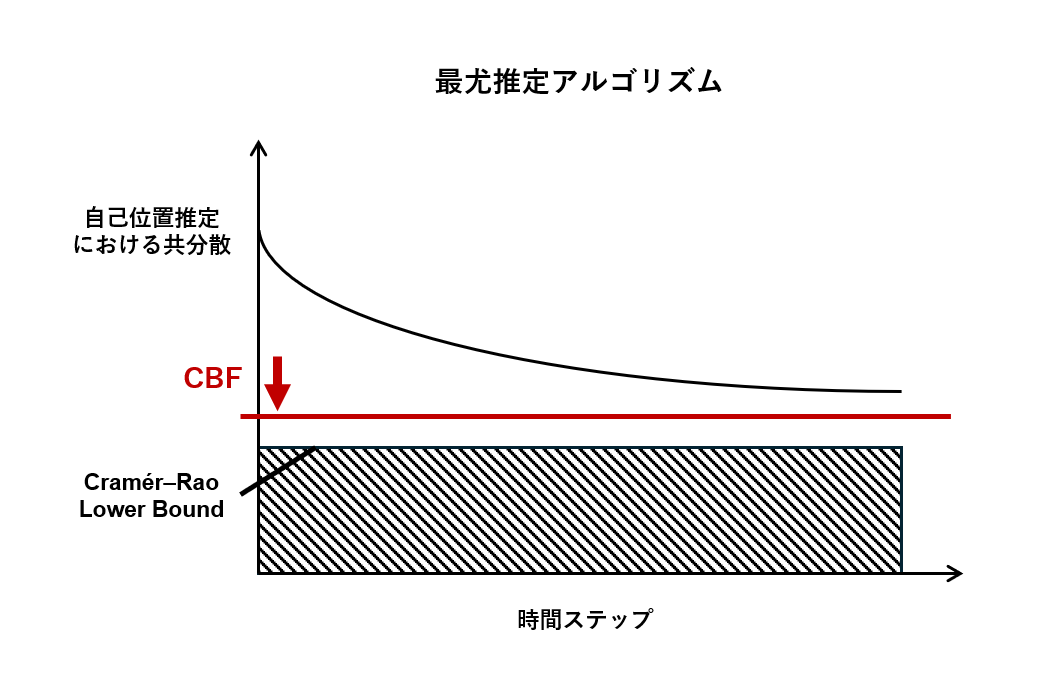
\includegraphics[width=0.7\linewidth]{fig/CRLB.png}
    \caption{クラメール・ラオの下限とCBFの関係}
    \label{fig:CRLB}
\end{figure}

\subsection{確率関数の時間微分と線形化}

確率関数をCBFに適用するには,確率関数の時間微分を制御入力$v_i, v_j$についての線形な関数に変換する必要がある.ここで
\begin{equation}
\begin{aligned}
\dot P_{ij}^l
&= -\frac{\sigma^2}{f^2}\,P_{ij}^l\,\dot T,\\
\dot T
&= \mathrm{tr}\left((M^{-1})^{\cdot}\right)
= -\mathrm{tr}\left(M^{-1}\dot M\,M^{-1}\right).
\end{aligned}
\label{eq:chain_rule}
\end{equation}

ただし$M$は各エージェント $k\in\{i,j\}$ の速度を $w_k=R_k v_k$ とし
\begin{equation}
\begin{aligned}
\dot M
&=\sum_{k\in\{i,j\}}
\frac{\mathrm d}{\mathrm dt}\left(\tfrac{P_{\beta_k}}{d_k^2}\right)\\
&=\sum_{k}
\frac{1}{d_k^2}\dot P_{\beta_k}
-\frac{2\dot d_k}{d_k^3}P_{\beta_k}\\
&=\sum_{k}
\frac{1}{d_k^3}\left[
P_{\beta_k}w_k\beta_k^\top
+\beta_k w_k^\top P_{\beta_k}
+2(\beta_k^\top w_k)P_{\beta_k}
\right].
\end{aligned}
\label{eq:Mdot}
\end{equation}
のように時間微分を計算することができる.

また,トレース演算は以下
\begin{equation}
\begin{aligned}
&\mathrm{tr}\left(M^{-1}\dot M\,M^{-1}\right)\\
&=\sum_{k\in\{i,j\}}
\frac{1}{d_k^3}\left[
\underbrace{\mathrm{tr}(M^{-1}P_{\beta_k}w_k\beta_k^\top M^{-1})}_{t_{k,1}}
+\underbrace{\mathrm{tr}(M^{-1}\beta_k w_k^\top P_{\beta_k}M^{-1})}_{t_{k,2}}
+\underbrace{2(\beta_k^\top w_k)\mathrm{tr}(M^{-1}P_{\beta_k}M^{-1})}_{t_{k,3}}
\right].
\end{aligned}
\label{eq:trace_expand}
\end{equation}
のように分解できる.ただし各項は
$\mathrm{tr}(A\,x\,y^\top\,B)=y^\top B A x$
により
\begin{equation}
\begin{aligned}
t_{k,1}&=w_k^\top P_{\beta_k}M^{-2}\beta_k,\\
t_{k,2}&=w_k^\top P_{\beta_k}M^{-2}\beta_k,\\
t_{k,3}&=2(\beta_k^\top w_k)\,\chi_k,\quad
\chi_k=\mathrm{tr}(M^{-1}P_{\beta_k}M^{-1}).
\end{aligned}
\label{eq:t_terms}
\end{equation}
を得る。よって
\begin{equation}
\begin{aligned}
\mathrm{tr}\left(M^{-1}\dot M\,M^{-1}\right)
&=\sum_{k}
\frac{2}{d_k^3}
w_k^\top\left(P_{\beta_k}M^{-2}\beta_k + \chi_k\beta_k\right).
\end{aligned}
\label{eq:trace_linear}
\end{equation}

上記の変形により,
\eqref{eq:chain_rule}, \eqref{eq:trace_linear} と $w_k=R_k v_k$ を組み合わせ,
\begin{equation}
\begin{aligned}
\dot P_{ij}^l
&=-\frac{\sigma^2}{f^2}P_{ij}^l\left(-\mathrm{tr}(M^{-1}\dot M\,M^{-1})\right)\\
&=\sum_{k\in\{i,j\}}
\lambda_k^\top v_k,
\end{aligned}
\label{eq:Pdot_prel}
\end{equation}
\[
\lambda_k
:=-\frac{2\sigma^2}{f^2}\,
\frac{P_{ij}^l}{d_k^3}\,
R_k^\top\left(P_{\beta_k}M^{-2}\beta_k + \chi_k\beta_k\right).
\]

最終的に
\begin{equation}
\begin{aligned}
\dot P_{ij}^l
= \lambda_i^\top v_i + \lambda_j^\top v_j
\end{aligned}
\label{eq:Pdot_linear}
\end{equation}
が得られる。以上で
$\dot P_{ij}^l$ がエージェント速度 $v_i,v_j$ に対し線形であることを示した。

今後の課題としては,今回シミュレーションを十分に検証できなかった2次系及び非ホロノミック系の結果検証の他,上記で示した自己位置推定における共分散を下限する確率関数の導入を行いたい.

\begin{thebibliography}{99}
\bibitem{Ames2017} A. D. Ames, X. Xu, J. W. Grizzle, and P. Tabuada, ``Control barrier function based quadratic programs for safety critical systems,'' {\it IEEE Transactions on Automatic Control}, Vol. 62, No. 8, pp. 3861-3876, 2017.

\bibitem{Arandjelovic2016} R. Arandjelovic, P. Gronat, A. Torii, T. Pajdla, and J. Sivic, ``NetVLAD: CNN architecture for weakly supervised place recognition,'' {\it Proceedings of the IEEE Conference on Computer Vision and Pattern Recognition}, pp. 5297-5307, 2016.

\bibitem{Capelli2020} B. Capelli and L. Sabattini, ``Connectivity maintenance: Global and optimized approach through control barrier functions,'' {\it Proceedings of the IEEE International Conference on Robotics and Automation (ICRA)}, pp. 5590-5596, 2020.

\bibitem{Chang2016} T.-H. Chang, M. Hong, W.-C. Liao, and X. Wang, ``Distributed optimization using the primal-dual method of multipliers,'' {\it IEEE Transactions on Signal Processing}, Vol. 64, No. 2, pp. 447-461, 2016.

\bibitem{DeTone2018} D. DeTone, T. Malisiewicz, and A. Rabinovich, ``SuperPoint: Self-supervised interest point detection and description,'' {\it Proceedings of the IEEE Conference on Computer Vision and Pattern Recognition Workshops}, pp. 224-236, 2018.

\bibitem{Dias2016} D. Dias, P. U. Lima, and A. Martinoli, ``Distributed Formation Control of Quadrotors under Limited Sensor Field of View,'' {\it Proceedings of the International Conference on Autonomous Agents and Multiagent Systems (AAMAS)}, pp. 1087-1095, 2016.

\bibitem{Jankovic2022} M. Jankovic, M. Egerstedt, and S. Coogan, ``Barrier functions for multiagent systems: An overview,'' {\it Annual Reviews in Control}, Vol. 53, pp. 329-348, 2022.

\bibitem{Lee2010} T. Lee, M. Leok, and N. H. McClamroch, ``Geometric tracking control of a quadrotor UAV on SE(3),'' {\it Proceedings of the IEEE Conference on Decision and Control}, pp. 5420-5425, 2010.

\bibitem{Lee2013} T. Lee, M. Leok, and N. H. McClamroch, ``Nonlinear robust tracking control of a quadrotor UAV on SE(3),'' {\it Asian Journal of Control}, Vol. 15, No. 2, pp. 391-408, 2013.

\bibitem{Lv2024} X. Lv, C. Peng, and J. Ma, ``Control Barrier Function-Based Collision Avoidance Guidance Strategy for Multi-Fixed-Wing UAV Pursuit-Evasion Environment,'' {\it Drones}, Vol. 8, No. 8, pp. 415, 2024.

\bibitem{Panagou2012} D. Panagou and V. Kumar, ``Maintaining visibility for leader-follower formations in obstacle environments,'' {\it Proceedings of the IEEE International Conference on Robotics and Automation (ICRA)}, pp. 1811-1816, 2012.

\bibitem{Panagou2017} D. Panagou, D. M. Stipanovic, and P. G. Voulgaris, ``Distributed dynamic coverage and avoidance control under anisotropic sensing,'' {\it IEEE Transactions on Control of Network Systems}, Vol. 4, No. 4, pp. 850-862, 2017.

\bibitem{Sabattini2013} L. Sabattini, C. Secchi, and N. Chopra, ``Decentralized control for the maintenance of strong connectivity for directed graphs,'' {\it Proceedings of the Mediterranean Conference on Control and Automation}, pp. 978-986, 2013.

\bibitem{Zhang2022} T. Zhang, L. Zhang, Y. Chen, and Y. Zhou, ``CVIDS: A collaborative localization and dense mapping framework for multi-agent based visual-inertial SLAM,'' {\it IEEE Transactions on Image Processing}, Vol. 31, pp. 6562-6576, 2022.

\bibitem{Tan2022} X. Tan and D. V. Dimarogonas, ``Distributed Implementation of Control Barrier Functions for Multi-agent Systems,'' {\it IEEE Control Systems Letters}, Vol. 6, pp. 1879-1884, 2022.

\bibitem{Taylor2020} A. J. Taylor, A. Singletary, Y. Yue, and A. D. Ames, ``Learning for safety-critical control with control barrier functions,'' {\it Proceedings of the 2nd Conference on Learning for Dynamics and Control}, pp. 708-717, 2020.

\bibitem{Trimarchi2025} B. Trimarchi, F. Schiano, and R. Tron, ``A Control Barrier Function Candidate for Quadrotors with Limited Field of View,'' {\it arXiv:2410.01277 [eess.SY]}, 2025.

\bibitem{Wang2017} Y. Wang, A. D. Ames, and M. Egerstedt, ``Safety barrier certificates for collisions-free multi-robot systems,'' {\it IEEE Transactions on Robotics}, Vol. 33, No. 3, pp. 641-652, 2017.

\bibitem{Xiao2022} W. Xiao and C. Belta, ``High-order control barrier functions,'' {\it IEEE Transactions on Automatic Control}, Vol. 67, No. 7, pp. 3655-3662, 2022.

\bibitem{Zhang2017} G. Zhang and R. Heusdens, ``Distributed Optimization Using the Primal-Dual Method of Multipliers (PDMM),'' {\it arXiv:1702.00841 [cs.DC]}, 2017.


\bibitem{Zhang2018} Z. Zhang and D. Scaramuzza, ``Perception-aware receding horizon navigation for MAVs,'' {\it Proceedings of the IEEE International Conference on Robotics and Automation (ICRA)}, pp. 2534-2541, 2018.
\end{thebibliography}


\end{document}
